%%%%%%%%%%%%%%%%%%%%%%%%%%%%%%%%%%%%%%%%%
% Masters/Doctoral Thesis 
% LaTeX Template
% Version 2.5 (27/8/17)
%
% This template was downloaded from:
% http://www.LaTeXTemplates.com
%
% Version 2.x major modifications by:
% Vel (vel@latextemplates.com)
%
% This template is based on a template by:
% Steve Gunn (http://users.ecs.soton.ac.uk/srg/softwaretools/document/templates/)
% Sunil Patel (http://www.sunilpatel.co.uk/thesis-template/)
%
% Template license:
% CC BY-NC-SA 3.0 (http://creativecommons.org/licenses/by-nc-sa/3.0/)
%
%%%%%%%%%%%%%%%%%%%%%%%%%%%%%%%%%%%%%%%%%

%----------------------------------------------------------------------------------------
%	PACKAGES AND OTHER DOCUMENT CONFIGURATIONS
%----------------------------------------------------------------------------------------

\documentclass[
11pt, % The default document font size, options: 10pt, 11pt, 12pt
%oneside, % Two side (alternating margins) for binding by default, uncomment to switch to one side
english, % ngerman for German
singlespacing, % Single line spacing, alternatives: onehalfspacing or doublespacing
%draft, % Uncomment to enable draft mode (no pictures, no links, overfull hboxes indicated)
%nolistspacing, % If the document is onehalfspacing or doublespacing, uncomment this to set spacing in lists to single
%liststotoc, % Uncomment to add the list of figures/tables/etc to the table of contents
%toctotoc, % Uncomment to add the main table of contents to the table of contents
%parskip, % Uncomment to add space between paragraphs
%nohyperref, % Uncomment to not load the hyperref package
headsepline, % Uncomment to get a line under the header
%chapterinoneline, % Uncomment to place the chapter title next to the number on one line
%consistentlayout, % Uncomment to change the layout of the declaration, abstract and acknowledgements pages to match the default layout
]{MastersDoctoralThesis} % The class file specifying the document structure

\usepackage[utf8]{inputenc} % Required for inputting international characters
\usepackage[T1]{fontenc} % Output font encoding for international characters

\usepackage{mathpazo} % Use the Palatino font by default

\usepackage[backend=bibtex,style=authoryear,natbib=true]{biblatex} % Use the bibtex backend with the authoryear citation style (which resembles APA)

\addbibresource{example.bib} % The filename of the bibliography

\usepackage[autostyle=true]{csquotes} % Required to generate language-dependent quotes in the bibliography

%----------------------------------------------------------------------------------------
%	MARGIN SETTINGS
%----------------------------------------------------------------------------------------

\geometry{
	paper=a4paper, % Change to letterpaper for US letter
	inner=2.5cm, % Inner margin
	outer=3.8cm, % Outer margin
	bindingoffset=.5cm, % Binding offset
	top=1.5cm, % Top margin
	bottom=1.5cm, % Bottom margin
	%showframe, % Uncomment to show how the type block is set on the page
}

%----------------------------------------------------------------------------------------
%	THESIS INFORMATION
%----------------------------------------------------------------------------------------

% The title, son. It's krill. It's GREAT. Make krill great again.
\thesistitle{Seasonal, Physiological and Genetic Functions in Antarctic Krill, \textit{Euphausia superba}, at Different Latitudes in the Southern Ocean} % Your thesis title, this is used in the title and abstract, print it elsewhere with \ttitle
\supervisor{Dr. Bettina \textsc{Meyer}} % Your supervisor's name, this is used in the title page, print it elsewhere with \supname
\examiner{} % Your examiner's name, this is not currently used anywhere in the template, print it elsewhere with \examname
\degree{Doktor der Naturwissenschaften} % Your degree name, this is used in the title page and abstract, print it elsewhere with \degreename
\author{Flavia \textsc{H{\"o}ring}} % Your name, this is used in the title page and abstract, print it elsewhere with \authorname
\addresses{} % Your address, this is not currently used anywhere in the template, print it elsewhere with \addressname

\subject{Biological Sciences} % Your subject area, this is not currently used anywhere in the template, print it elsewhere with \subjectname
\keywords{} % Keywords for your thesis, this is not currently used anywhere in the template, print it elsewhere with \keywordnames
\university{\href{http://www.university.com}{University Name}} % Your university's name and URL, this is used in the title page and abstract, print it elsewhere with \univname
\department{\href{http://department.university.com}{Department or School Name}} % Your department's name and URL, this is used in the title page and abstract, print it elsewhere with \deptname
\group{\href{http://researchgroup.university.com}{Research Group Name}} % Your research group's name and URL, this is used in the title page, print it elsewhere with \groupname
\faculty{\href{http://faculty.university.com}{Faculty Name}} % Your faculty's name and URL, this is used in the title page and abstract, print it elsewhere with \facname

\AtBeginDocument{
\hypersetup{pdftitle=\ttitle} % Set the PDF's title to your title
\hypersetup{pdfauthor=\authorname} % Set the PDF's author to your name
\hypersetup{pdfkeywords=\keywordnames} % Set the PDF's keywords to your keywords
}
\linespread{1.5}
\begin{document}

\frontmatter % Use roman page numbering style (i, ii, iii, iv...) for the pre-content pages

\pagestyle{plain} % Default to the plain heading style until the thesis style is called for the body content

%----------------------------------------------------------------------------------------
%	TITLE PAGE
%----------------------------------------------------------------------------------------

\begin{titlepage}
\begin{center}

\vspace*{.06\textheight}
{\scshape\LARGE \univname\par}\vspace{1.5cm} % University name
\textsc{\Large Doctoral Thesis}\\[0.5cm] % Thesis type

\HRule \\[0.4cm] % Horizontal line
{\huge \bfseries \ttitle\par}\vspace{0.4cm} % Thesis title
\HRule \\[1.5cm] % Horizontal line
 
\begin{minipage}[t]{0.4\textwidth}
\begin{flushleft} \large
\emph{Author:}\\
\href{http://www.johnsmith.com}{\authorname} % Author name - remove the \href bracket to remove the link
\end{flushleft}
\end{minipage}
\begin{minipage}[t]{0.4\textwidth}
\begin{flushright} \large
\emph{Supervisor:} \\
\href{http://www.jamessmith.com}{\supname} % Supervisor name - remove the \href bracket to remove the link  
\end{flushright}
\end{minipage}\\[3cm]
 
\vfill

\large \textit{A thesis submitted in fulfillment of the requirements\\ for the degree of \degreename}\\[0.3cm] % University requirement text
\textit{in the}\\[0.4cm]
\groupname\\\deptname\\[2cm] % Research group name and department name
 
\vfill

{\large \today}\\[4cm] % Date
%\includegraphics{Logo} % University/department logo - uncomment to place it
 
\vfill
\end{center}
\end{titlepage}

%----------------------------------------------------------------------------------------
%	DECLARATION PAGE
%----------------------------------------------------------------------------------------

\begin{declaration}
\addchaptertocentry{\authorshipname} % Add the declaration to the table of contents
\noindent I, \authorname, declare that this thesis titled, \enquote{\ttitle} and the work presented in it are my own. I confirm that:

\begin{itemize} 
\item This work was done wholly or mainly while in candidature for a research degree at this University.
\item Where any part of this thesis has previously been submitted for a degree or any other qualification at this University or any other institution, this has been clearly stated.
\item Where I have consulted the published work of others, this is always clearly attributed.
\item Where I have quoted from the work of others, the source is always given. With the exception of such quotations, this thesis is entirely my own work.
\item I have acknowledged all main sources of help.
\item Where the thesis is based on work done by myself jointly with others, I have made clear exactly what was done by others and what I have contributed myself.\\
\end{itemize}
 
\noindent Signed:\\
\rule[0.5em]{25em}{0.5pt} % This prints a line for the signature
 
\noindent Date:\\
\rule[0.5em]{25em}{0.5pt} % This prints a line to write the date
\end{declaration}

\cleardoublepage

%----------------------------------------------------------------------------------------
%	QUOTATION PAGE
%----------------------------------------------------------------------------------------

\vspace*{0.2\textheight}

\noindent\enquote{\itshape Thanks to my solid academic training, today I can write hundreds of words on virtually any topic without possessing a shred of information, which is how I got a good job in journalism.}\bigbreak

\hfill Dave Barry

%----------------------------------------------------------------------------------------
%	ABSTRACT PAGE
%----------------------------------------------------------------------------------------

\begin{abstract}
\addchaptertocentry{\abstractname} % Add the abstract to the table of contents
The Thesis Abstract is written here (and usually kept to just this page). The page is kept centered vertically so can expand into the blank space above the title too\ldots
\end{abstract}

%----------------------------------------------------------------------------------------
%	ACKNOWLEDGEMENTS
%----------------------------------------------------------------------------------------

\begin{acknowledgements}
\addchaptertocentry{\acknowledgementname} % Add the acknowledgements to the table of contents
The acknowledgments and the people to thank go here, don't forget to include your project advisor\ldots
\end{acknowledgements}

%----------------------------------------------------------------------------------------
%	LIST OF CONTENTS/FIGURES/TABLES PAGES
%----------------------------------------------------------------------------------------

\tableofcontents % Prints the main table of contents

\listoffigures % Prints the list of figures

\listoftables % Prints the list of tables

%----------------------------------------------------------------------------------------
%	ABBREVIATIONS
%----------------------------------------------------------------------------------------

\begin{abbreviations}{ll} % Include a list of abbreviations (a table of two columns)

\textbf{LAH} & \textbf{L}ist \textbf{A}bbreviations \textbf{H}ere\\
\textbf{WSF} & \textbf{W}hat (it) \textbf{S}tands \textbf{F}or\\

\end{abbreviations}

%----------------------------------------------------------------------------------------
%	PHYSICAL CONSTANTS/OTHER DEFINITIONS
%----------------------------------------------------------------------------------------

\begin{constants}{lr@{${}={}$}l} % The list of physical constants is a three column table

% The \SI{}{} command is provided by the siunitx package, see its documentation for instructions on how to use it

Speed of Light & $c_{0}$ & \SI{2.99792458e8}{\meter\per\second} (exact)\\
%Constant Name & $Symbol$ & $Constant Value$ with units\\

\end{constants}

%----------------------------------------------------------------------------------------
%	SYMBOLS
%----------------------------------------------------------------------------------------

\begin{symbols}{lll} % Include a list of Symbols (a three column table)

$a$ & distance & \si{\meter} \\
$P$ & power & \si{\watt} (\si{\joule\per\second}) \\
%Symbol & Name & Unit \\

\addlinespace % Gap to separate the Roman symbols from the Greek

$\omega$ & angular frequency & \si{\radian} \\

\end{symbols}

%----------------------------------------------------------------------------------------
%	DEDICATION
%----------------------------------------------------------------------------------------

\dedicatory{For/Dedicated to/To my\ldots} 

%----------------------------------------------------------------------------------------
%	THESIS CONTENT - CHAPTERS
%----------------------------------------------------------------------------------------

\mainmatter % Begin numeric (1,2,3...) page numbering

\pagestyle{thesis} % Return the page headers back to the "thesis" style

% Include the chapters of the thesis as separate files from the Chapters folder
% Uncomment the lines as you write the chapters

% Chapter 1

\chapter{Introduction} % Main chapter title

\label{Intro} % For referencing the chapter elsewhere, use \ref{Chapter1} 

%----------------------------------------------------------------------------------------

% Define some commands to keep the formatting separated from the content 
\newcommand{\keyword}[1]{\textbf{#1}}
\newcommand{\tabhead}[1]{\textbf{#1}}
\newcommand{\code}[1]{\texttt{#1}}
\newcommand{\file}[1]{\texttt{\bfseries#1}}
\newcommand{\option}[1]{\texttt{\itshape#1}}
\newcommand{\krilllatin}{\textit{Euphausia superba}}
\newcommand{\krilllatinshort}{\textit{E. superba}}
%----------------------------------------------------------------------------------------

In this section, I would like to introduce the scientific background for this
dissertation which studied seasonal, physiological and genetic functions in
Antarctic krill, \textit{Euphausia superba}, under different latitudinal light
regimes. First, I will explain the importance of \textit{E. superba} in the
Southern Ocean ecosystem, the impact of fisheries, as well as the effects of
climate change and potential phenological mismatches on this species.
Afterwards, I will summarize findings from field studies that show that
Antarctic krill has evolved pronounced seasonal cycles of physiology and
behaviour to adapt to the highly variable environment in the Southern Ocean.
Then, I will integrate information about the seasonal timing system in
Antarctic krill including the role of environmental cues, the potential
mechanisms of the endogenous timing system and the neuroendocrine control. In a
final step, I will explain the gaps of knowledge, the research objectives of
this dissertation, and the methodological approach.

\section*{\textit{Euphausia superba}, a key organism in the Southern Ocean}
With an estimated circumpolar biomass of 379 Mt (Atkinson et al., 2009),
Antarctic krill (\textit{Euphausia superba} Dana, 1850) belongs to one of the
most abundant organisms on Earth. Antarctic krill is a key organism in the
Southern Ocean food web linking primary production to higher trophic levels
such as whales, penguins, birds and seals (Fig. 1). \textit{Euphausia superba}
is distributed over a large latitudinal range from approximately $50^{\circ}$S
to more than $70^{\circ}$S (Hill et al., 2013). These different latitudinal
habitats are characterized by extreme seasonal and regional fluctuations of
photoperiod, primary production and sea ice extent (Quetin and Ross, 1991).
Since Antarctic krill is able to travel great distances within one year, either
by active migration (Siegel, 1988) or passive transport within ocean currents
(Thorpe et al., 2007), it seems to be highly flexible in adjusting it's
phenology to both the high annual and regional variability of environmental
factors in the different latitudinal habitats of the Southern Ocean. 


\begin{figure}
        \caption{a) Simplified version of the Antarctic food web by Balana
        (2013) licenced under CC BY-NC-ND 3.0 ES; b) Latitudinal light regimes
        in different regions of the Southern Ocean by Meyer (2012) licenced
        under CC BY 4.0.}
        \centering
        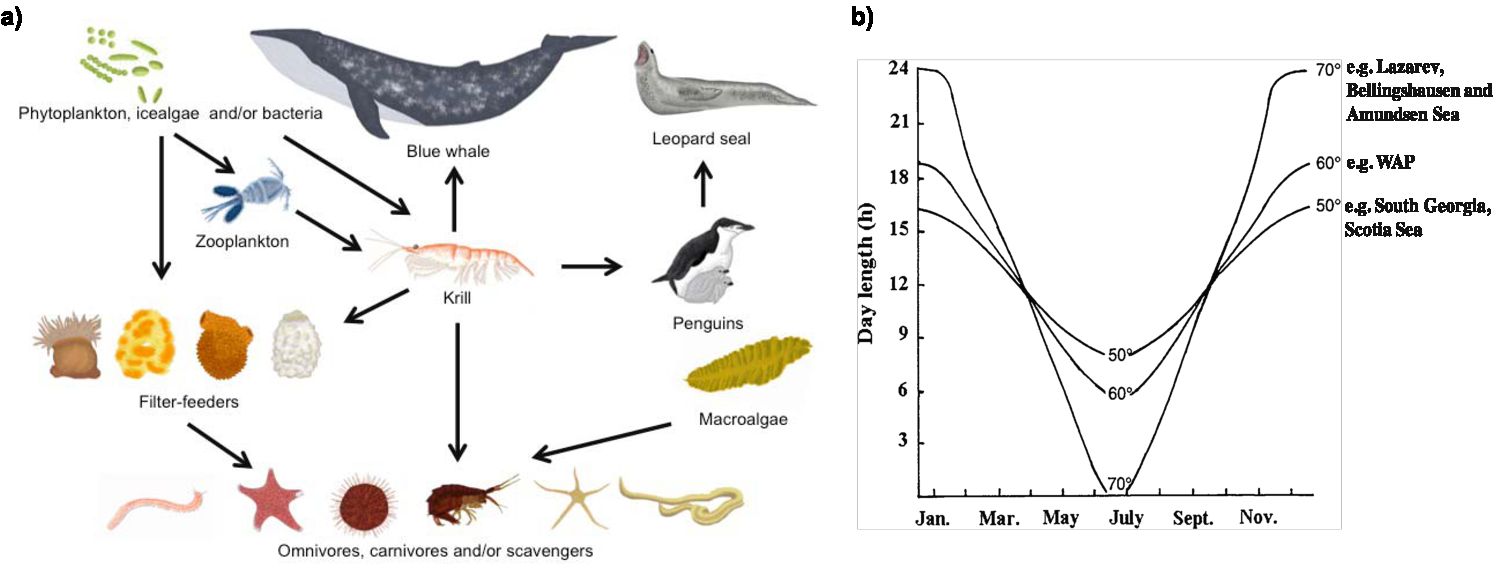
\includegraphics[width=0.85\textwidth]{../Figures/Figure1.pdf}
\end{figure}


Commercial interest in Antarctic krill and fishery are growing considering its
high biomass, improved harvesting techniques and the increasing demand for
newly developed krill products (Nicol et al., 2012). Antarctic krill is
considered of high nutritional value when used as 'krill meal' in aquaculture
(Yoshitomi et al., 2007) and for the production of dietary supplements and
pharmaceutical products because of their suggested beneficial properties for
human health (Tou et al., 2008). Krill fishery in the Southern Ocean is
currently managed by the Commission for the Conservation of Antarctic Marine
Living Resources (CCAMLR). However, sustainable fishery's management is largely
dependent on our current understanding of the Southern Ocean ecosystem and the
correct prediction of krill abundances under changing environmental conditions
in the future. 

Climate change may pose another threat to Antarctic krill. It has been
predicted that global warming and associated changes in chlorophyll
concentration will reduce the favourable growth habitat of Antarctic krill, and
thereby its biomass in the Southern Ocean (Hill et al., 2013). In the Southwest
Atlantic Sector, it has been reported that Antarctic krill densities have
declined associated with a southward shift of \textit{E. superba}'s
distribution and an increase in salp densities in that region (Atkinson et al.,
2004, 2019). This shift has been explained by changes in sea ice extent
(Atkinson et al., 2004) and anomalies of the Southern Annular Mode (Atkinson et
al., 2019). Changes in Antarctic krill biomass have been linked to the survival
of upper-level predators such as penguins which indicates that climate change
may lead to profound changes in the Southern food web (Trivelpiece et al.,
2011).

Climate change effects in the Southern Ocean are especially relevant under the
match/mismatch hypothesis that describes how the seasonal timing of a predator
and the availability of its prey may affect recruitment, reproduction or
survival of the predator (Durant et al., 2007). In particular, Antarctic krill
may be influenced by temporal and spatial changes in phytoplankton distribution
that do not match its seasonal requirements for recruitment or reproductive
processes. However, these effects are difficult to predict, because the
mechanisms and the flexibility of Antarctic krill's seasonal timing system are
poorly understood.

\section*{Pronounced Seasonal Cycles of \textit{E. superba} in the Field}

Pronounced seasonal variations of growth, feeding, metabolic activity (Meyer et
al., 2010), lipid turnover (Ericson et al., 2018; Hellessey et al., 2018),
reproduction (Siegel, 2012) and gene expression (Seear et al., 2012) have been
observed in Antarctic krill in the field (Fig. 2). Antarctic krill has evolved
different overwintering strategies to cope with the conditions of near-constant
darkness and low food availability in some regions of the Southern Ocean
(Meyer, 2012). The by far most important strategy is the reduction of
physiological functions consistent with a state of quiescence observed in
Antarctic krill. Respiration is severely reduced during the winter season and
may drop down to 30\% of the summer rates (Meyer et al., 2010; Quetin and Ross,
1991). Moreover, a significantly lower activity of the metabolic key enzymes
citrate synthase (Cullen et al., 2003; Meyer et al., 2002) and malate
dehydrogenase (Meyer et al., 2010; Pape et al., 2008) was found in autumn and
winter. In the course of winter-metabolic depression, low feeding activity has
been observed, with indications that Antarctic krill can switch to alternative
food sources like zooplankton or ice-algae (Atkinson et al., 2002; Meyer et
al., 2010). As a consequence, growth rates of adult krill are extremely reduced
during winter (Kawaguchi et al., 1986; Meyer et al., 2010), even shrinkage has
been reported (Quetin and Ross, 1991). The seasonal accumulation of lipid
stores and their utilisation during winter promotes survival of adult krill
during periods of low food availability (Falk-Petersen et al., 2000; Hagen et
al., 2001; Meyer et al., 2010; Quetin and Ross, 1991). Moreover, Antarctic
krill shows a pronounced seasonal cycle of maturity which is characterized by
the regression of its external sexual traits towards winter and the sexual
re-maturation towards spring (Kawaguchi et al., 2007). Gene expression analysis
of seasonal Antarctic krill samples near the Antarctic Peninsula revealed an
upregulation of genes related to feeding and digestion, respiration, motor
activity, immunity and vitellogenesis in summer krill with respect to winter
(Seear et al., 2012).

% Figure 2
\begin{figure}
        \caption{Schematic representation of seasonal cycles of photoperiod and
        primary production in the Southern Ocean, and sexual maturity,
        respiration and lipid content of Antarctic krill following information
        from Meyer 2012, Arrigo et al. 2008, Kawaguchi et al. 2007, and
        Hellessey et al. 2018}
        \centering
        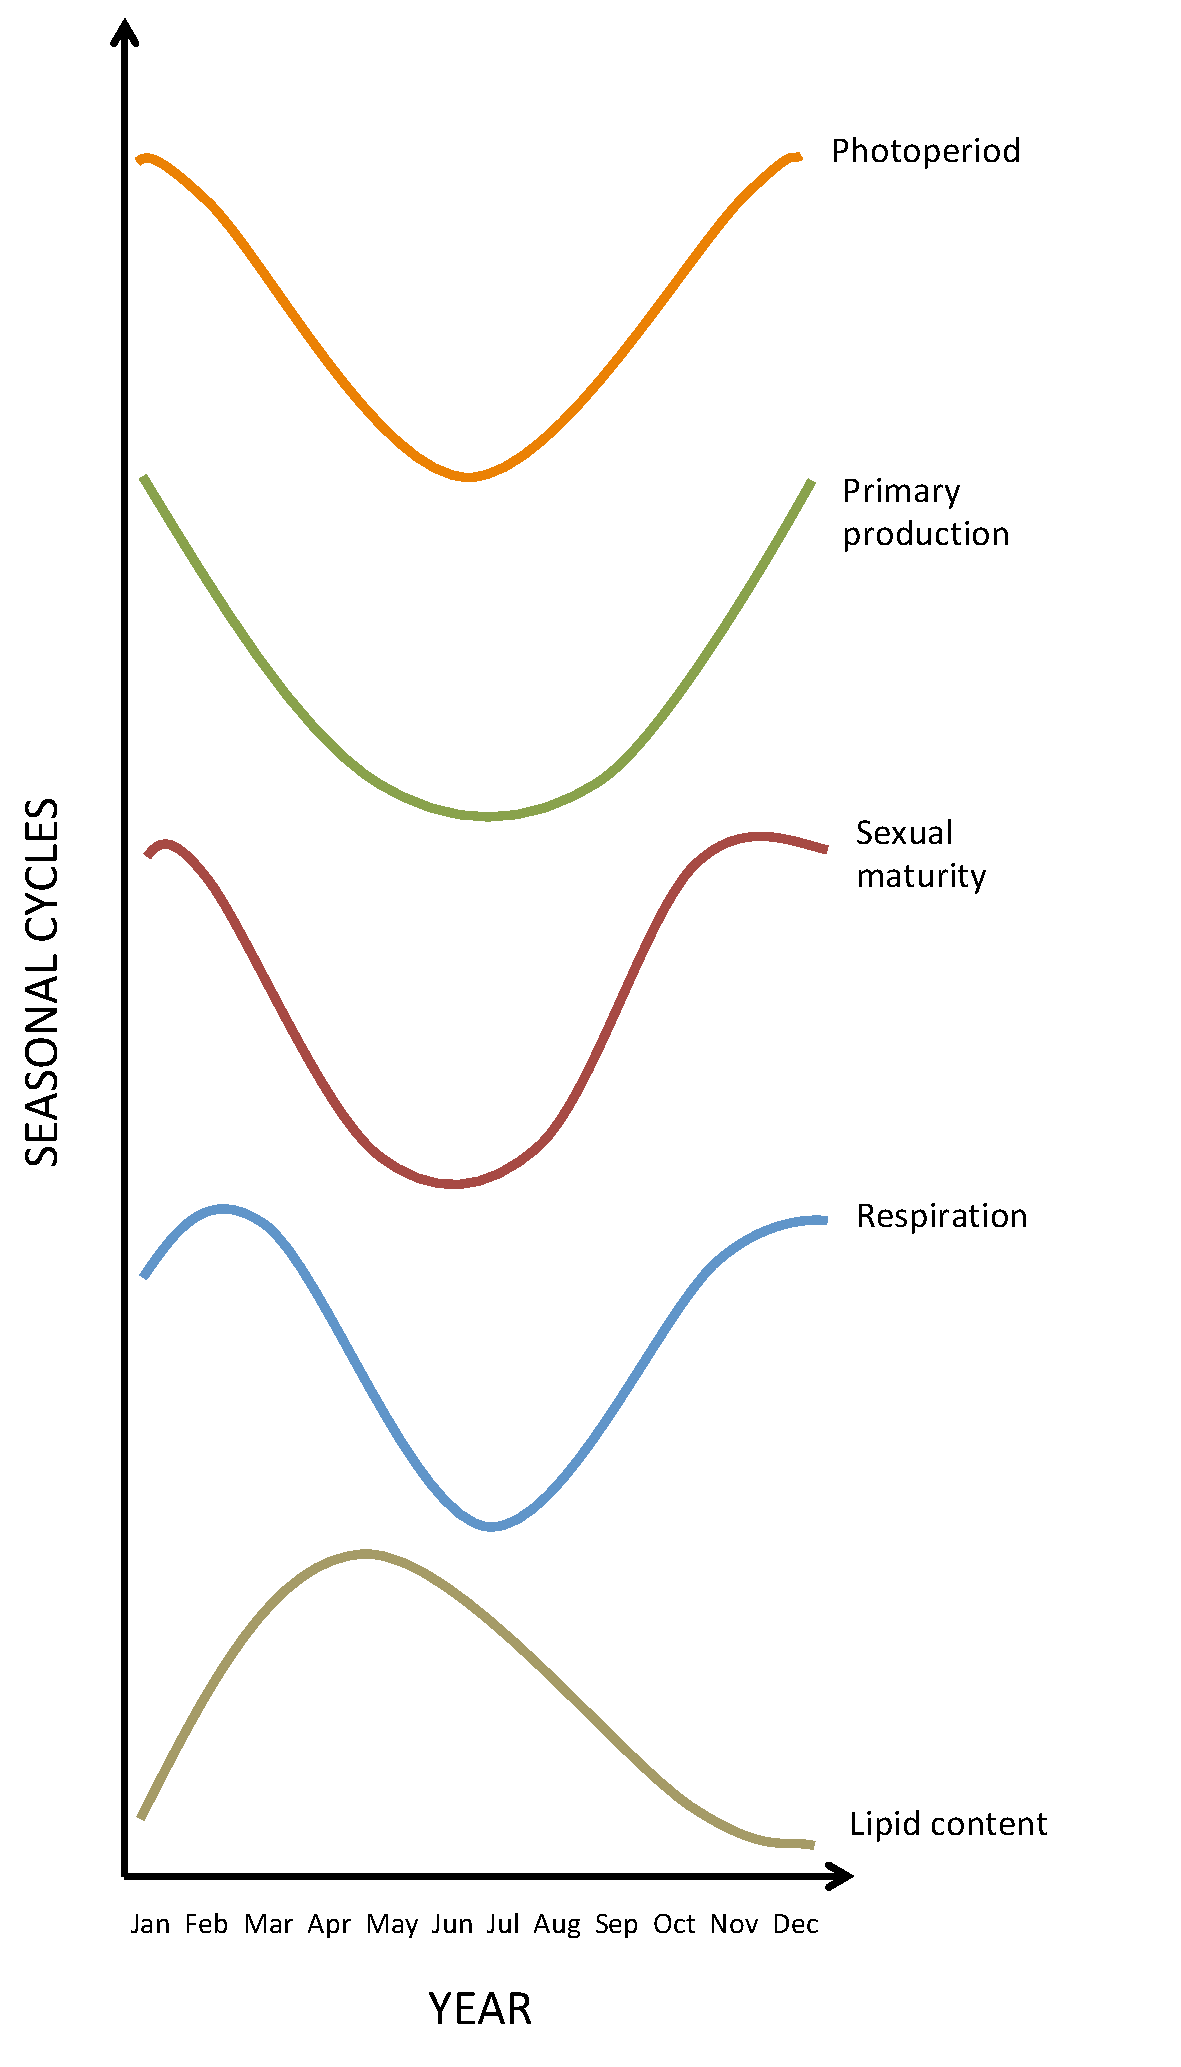
\includegraphics[width=0.85\textwidth]{../Figures/Figure2.pdf}
\end{figure}

Antarctic krill is able to synchronize its seasonal life cycle to local
photoperiod and food supply in the different latitudinal habitats of the
Southern Ocean. Regional differences in the timing of reproduction (Spiridonov,
1995), growth (Kawaguchi et al., 2006), feeding activity and lipid storage
(Schmidt et al., 2014), and gene expression (Seear et al., 2012) have been
observed in the field. Spiridonov (1995) investigated the spawning season of
Antarctic krill in different regions of the Southern Ocean and discussed that
the reproductive timing is largely dependent on the variation of  seasonal sea
ice cover and the timing of phytoplankton blooms. 

Kawaguchi et al. (2006) reported differences in the growth period of Antarctic
krill examining the Southwest Atlantic Sector and the Indian Ocean sector. The
authors suggested that the earlier timing of the phytoplankton bloom at lower
latitudes might advance the growth period of Antarctic krill. Differences in
the overwintering behaviour of Antarctic krill were observed by Schmidt et al.
(2014) and Seear et al. (2012) in different latitudinal habitats of the
Southern Ocean. Antarctic krill from the low-latitude region South Georgia had
higher feeding activities and lower lipid stores during winter compared to the
high-latitude region Lazarev Sea where Antarctic krill experienced
near-constant darkness and the strongest limitation in food supply (Schmidt et
al., 2014). Similar differences were found on the gene expression level, where
winter Antarctic krill from South Georgia showed higher gene activities related
to feeding, digestion and immunity with respect to krill from the Antarctic
Peninsula (Seear et al., 2012).

\section*{Seasonal timing mechanisms in \textit{E. superba}}

The variable light, food, and temperature regimes may play a role in the
regulation of \textit{E. superba}'s seasonal cycles in the different latitudinal
habitats of the Southern Ocean (Fig. 3). Controlled laboratory experiments were
conducted to unravel the specific effects of these parameters on the different
seasonal processes in Antarctic krill. Higher water temperatures and high food
supply were found to increase the growth rates of Antarctic krill (Brown et
al., 2010; Buchholz, 1991), whereas seasonal changes of photoperiod modulated a
seasonal growth pattern (Piccolin et al., 2018a). Kawaguchi et al. (2007) found
that favourable feeding conditions accelerate the sexual maturation process of
Antarctic krill. The initiation of sexual maturation and spawning were also
observed when exposing Antarctic krill to long photoperiods (Hirano et al.,
2003; Teschke et al., 2008). These long photoperiodic conditions also triggered
an enhanced lipid catabolism that was suggested to be necessary for the
maturation process (Teschke et al., 2008). During long-term laboratory
experiments of constant food supply, different simulated light regimes flexibly
adjusted the seasonal cycle of maturity in Antarctic krill (Brown et al.,
2011). The metabolic activity of Antarctic krill was observed to be higher
under long photoperiods similar to summer and autumn conditions compared to the
simulated winter condition 'constant darkness' (Teschke et al., 2007), while
the same study indicated that Antarctic krill might not be able to respond to
high food concentrations under constant darkness. Although food supply and
temperature have the potential to affect the respiration rates of Antarctic
krill, these factors do not change the general seasonal pattern of metabolic
activity (Brown et al., 2013). Recently, Piccolin et al. (2018a) confirmed in
long-term experiments that a simulated annual light regime could trigger the
seasonal cycle of metabolic activity in Antarctic krill. These seasonal
photoperiodic effects on krill's metabolic cycle were also found on gene
expression level (Piccolin et al., 2018a; Seear et al., 2009). 

% Figure 3

\begin{figure}
        \caption{Schematic representation of the seasonal timing system of Antarctic krill.}
        \centering
        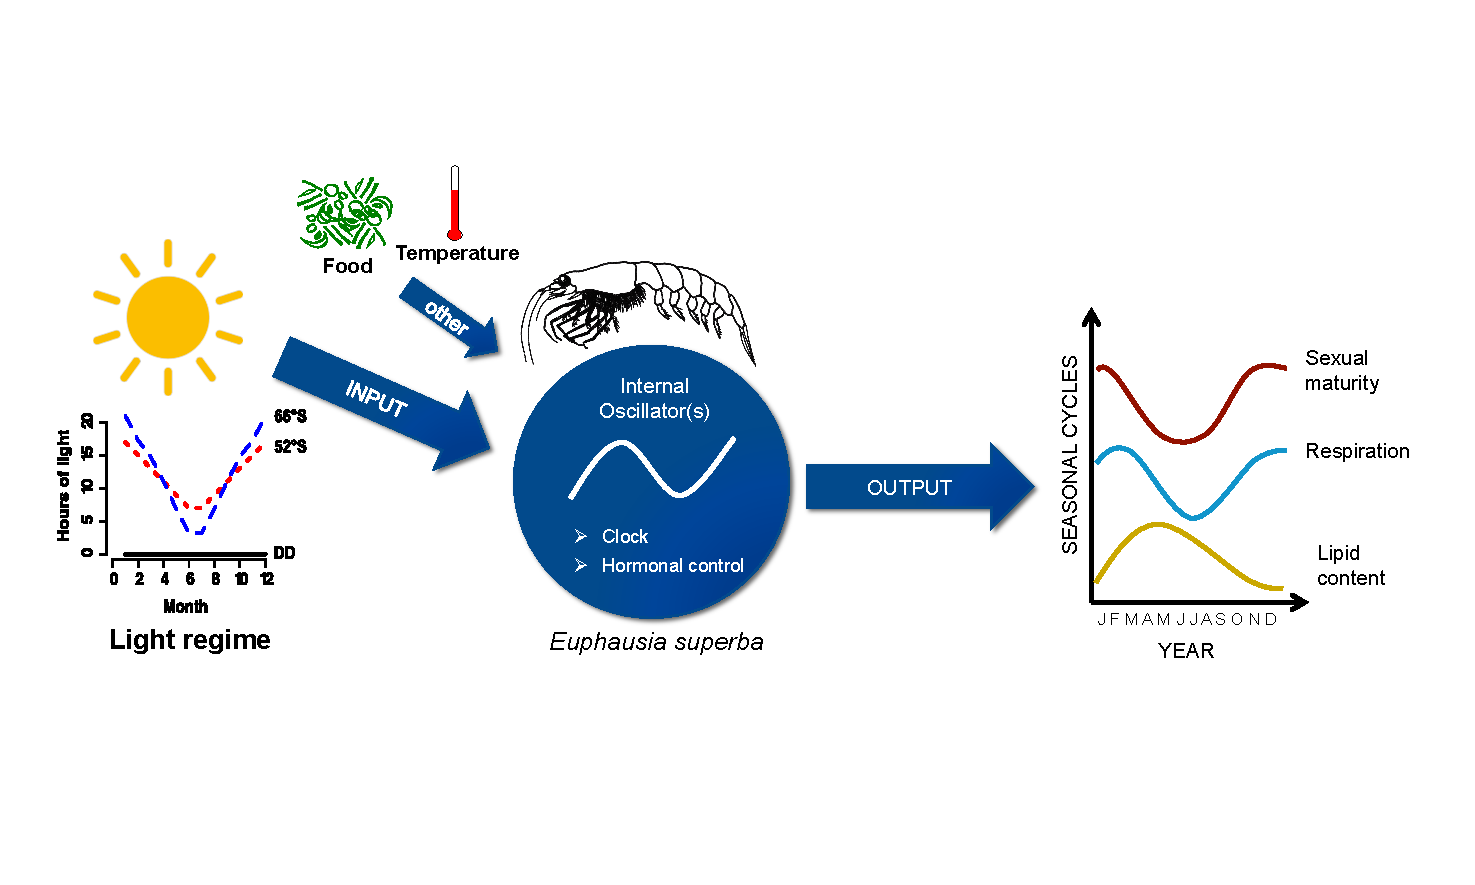
\includegraphics[width=0.85\textwidth]{../Figures/Figure3.pdf}
\end{figure}

These studies reveal that light regime and seasonal changes in photoperiod are
major cues that entrain the seasonal rhythms of growth, maturity, metabolic
activity and gene expression in Antarctic krill. It has been suggested that
these seasonal rhythms are controlled by an endogenous timing system with
photoperiod as timing cue (zeitgeber) (Brown et al., 2011, 2013; Piccolin et
al., 2018a). An endogenous timing system (circannual clock) is characterized by
the observation that seasonally rhythmic patterns persist, even if the actual
zeitgeber is not present (Visser et al., 2010). Such evidence was found in
Antarctic krill during long-term laboratory experiments where seasonal patterns
of maturity, growth and metabolic activity were observed under constant
darkness (Brown et al., 2011, 2013; Piccolin et al., 2018a).

In general, the molecular mechanisms of seasonal timing systems are poorly
understood, but there are indications that the circadian (daily) clock may play
role for photoperiodic time measurement and consequently the timing of seasonal
life cycle events (Helm et al., 2013). In eukaryotes, the circadian clock
functions as an approximately 24-h oscillator via interlaced
transcriptional/posttranslational feedback loops that are synchronized by an
environmental factor such as photoperiod (Mackey, 2007). In insects, circadian
clock genes were found to play an important role for the seasonal photoperiodic
timing of diapause (review by Goto, 2013; Meuti and Denlinger, 2013; Meuti et
al., 2015), with exceptions (e.g. Emerson et al., 2009). The investigation of
latitudinal clines of photoperiodism showed that insect populations generally
showed higher critical photoperiods for the initiation of diapause at higher
latitudes, and latitudinal adaptation of their photoperiodic response has been
linked to clock gene polymorphisms (Hut et al., 2013). Photoperiodic plasticity
may also be based on the differential expression of clock genes (Hodkova et
al., 2003) depending on season and latitude. Moreover, it is speculated, if
non-coding RNA or epigenetic modifications play a role in the regulation of
circannual rhythms (Helm and Stevenson, 2014).

In Antarctic krill, molecular studies have analysed the functioning of its
visual perception system and its circadian clock (Biscontin et al., 2016,
2017). Different opsin genes were identified in Antarctic krill that are
important for the visual perception of light of different wavelengths
(Biscontin et al., 2016). The circadian clock machinery of Antarctic krill was
characterized by Biscontin et al. (2017) who found that the core clock
resembled both insect's and mammalian circadian clock systems with a light
mediated degradation mechanism that suggested light as the main zeitgeber.
Controlled laboratory experiments revealed that the daily oscillations of clock
genes in Antarctic krill varied under variable seasonal conditions of
photoperiod and became arrhythmic under mid-winter and mid-summer conditions
(Piccolin et al., 2018b). Antarctic krill's circadian clock has not only been
linked to the timing of daily rhythms of metabolic activity (De Pittà et al.,
2013; Piccolin et al., 2018b; Teschke et al., 2011) and diel vertical migration
(Gaten et al., 2008), but it is also suggested to play a role for the seasonal
day length measurement and the regulation of seasonal rhythms in Antarctic
krill based on the observation of seasonal patterns of clock gene expression in
Antarctic krill (Piccolin et al., 2018a). 

In crustaceans, circadian pacemakers (clocks) are located in the nervous
system, in particular in retina of the eye, the eyestalk, the brain and the
caudal photoreceptor (Arechiga and Rodriguez-Sosa, 2002; Rodríguez‐Sosa et al.,
2008) and may be linked to neuroendocrine control of seasonal rhythms. Seasonal
life cycle events in decapods are mediated by various neuropeptides and
signalling molecules that originate from the X-organ-sinus gland system of the
eyestalk ganglia, brain, the thoracic ganglia, the Y-organ and the mandibular
organ (Nagaraju, 2011). Important hormones comprise the 'CHH-superfamily'
including the crustacean hyperglycaemic hormone, the moult-inhibiting hormone,
the gonad/vitellogenesis-inhibiting hormone and the mandibular organ-inhibiting
hormone that have multiple functions in carbohydrate and lipid metabolism,
reproduction, moulting, osmoregulation and the regulation of methyl farnesoate
synthesis from the mandibular organ (review by Webster et al., 2012). Other
hormones that control moulting and reproduction in crustaceans include methyl
farnesoate (Reddy et al., 2004), ecdysteroids and 'vertebrate-type' steroids
(Lafont and Mathieu, 2007), and prostaglandins (review by Nagaraju, 2011).

In Antarctic krill, studies on the neuroendocrine control of seasonal processes
are rare (Buchholz, 1991; Pape et al., 2008; Seear et al., 2012; Toullec et
al., 2013). Buchholz (1991) studied changes in hemolymph titre of
ecdysone-equivalents in the different moult stages of Antarctic krill. Pape et
al. (2008) were not able to detect melatonin in Antarctic krill and therefore
rejected the hypothesis that it played a role in regulating the seasonal
metabolic cycle of Antarctic krill (Teschke et al., 2007).  In the field,
seasonal gene expression patterns of the neuropeptide neuroparsin and
insulin-like peptides have been discussed in relation to the seasonal
reproductive physiology of Antarctic krill (Seear et al., 2012). In the ice
krill, Euphausia crystallorophias, various neuropeptide hormones were
identified including members of the CHH superfamily (Toullec et al., 2013). The
recently developed transcriptome database may provide a source for \textit{E
superba}-specific target sequences of neuropeptides (Sales et al., 2017). 

\section*{Research objectives}
The current environmental changes in the Southern Ocean and the increasing
commercial interest in Antarctic krill emphasise the need to better understand
the adaptability of \textit{E. superba} in different latitudinal regions of the
Southern Ocean, especially under the aspect of potential mismatches in
biological timing. It has not yet been investigated, if different latitudinal
light regimes regulate the flexible seasonal physiology and behaviour of
Antarctic krill in its diverse latitudinal habitats.  In general, the seasonal
timing system of Antarctic krill is not well understood including the potential
involvement of the circadian clock and the neuroendocrine control of seasonal
rhythms in Antarctic krill. Laboratory experiments that observe the seasonal
cycle of Antarctic krill under controlled photoperiodic conditions over a
period of multiple years and simulating different latitudinal light regimes are
still lacking.

This dissertation aimed to understand the role of different latitudinal light
regimes on the seasonal cycle of Antarctic krill focussing on (a) the molecular
characterization of seasonal rhythms in different latitudinal habitats in the
field (Publication 1), and (b) the investigation of seasonal rhythms under a
two-year photoperiodic-controlled laboratory experiment with constant food
supply (Publication 2 \& 3). The following research objectives were addressed
in the three different chapters of the dissertation:

\begin{enumerate}
\item Investigation of seasonal and regional differences in gene expression of
        summer and winter Antarctic krill from three different latitudinal
                regions: South Georgia ($54^{\circ}$S), South
                Orkneys/Bransfield Strait ($60^{\circ}$S-$63^{\circ}$S) and
                Lazarev Sea ($62^{\circ}$S-$66^{\circ}$S) (Publication 1)
\item Analysis of seasonal cycles of growth, feeding, lipid metabolism and
        maturity of Antarctic krill under the simulated light regimes
                $52^{\circ}$S, $66^{\circ}$S, and constant darkness
                (Publication 2)
\item Characterization of seasonal expression patterns of genes involved in
        different metabolic processes, seasonal timing, reproduction, feeding
                and development under the simulated light regimes
                $52^{\circ}$S, $66^{\circ}$S, and constant darkness
                (Publication 3)
\end{enumerate}

A range of different methods were implemented to investigate the effect of
latitudinal light regime on Antarctic krill. An RNAseq approach was used to
characterize the seasonal and latitudinal gene expression differences in
Antarctic krill in the field and to identify suitable seasonal target genes
with focus on genes with potential regulatory functions in the seasonal cycle
of Antarctic krill. For the first time, a two-year laboratory experiment was
conducted that simulated different latitudinal light regimes and constant food
supply. Antarctic krill from the laboratory experiments was investigated using
morphometric and lipid content analysis, and gene expression data from custom
designed TaqMan cards.

The findings of this dissertation improve our understanding of the effect of
different latitudinal light regimes on seasonal cycles in Antarctic krill and
their underlying molecular mechanisms.

\chapter[Publication I]{Publication I}

\section*{Seasonal gene expression profiling of Antarctic krill
in three different latitudinal regions}

Flavia Höring, Lars Harms, Cristiano De Pittà, Gabriele Sales, Christian Reiss,
Bettina Meyer
% TODO: Affiliations
\begin{center}
Ready to be submitted to the journal Marine Genomics
\end{center}

\section{Abstract}

The key organism Antarctic krill, \textit{Euphausia superba}, has evolved
seasonal rhythms of physiology and behaviour to survive under the extreme
photoperiodic conditions in the Southern Ocean. However, the molecular
mechanisms generating these rhythms remain far from understood. The aim of this
study was to investigate seasonal and regional differences in gene expression
in three different latitudinal regions with variable photoperiodic conditions
(South Georgia, South Orkneys/Bransfield Strait, Lazarev Sea) and to identify
genes with potential regulatory roles in the seasonal life cycle of Antarctic
krill. The RNAseq data were analysed (a) for seasonal differences between
summer and winter field samples from each region, and (b) for regional
differences within each season. In general, we found an upregulation of gene
expression in summer krill in all regions with respect to winter.  However,
seasonal differences in gene expression were less pronounced in Antarctic krill
from South Georgia where most genes related to metabolic, biological and
regulatory processes were not found to be differentially expressed between
summer and winter krill. We also identified genes with putative regulatory
roles, for instance genes related to hormone metabolism and signalling,
reproductive and developmental processes. Our results suggest that Antarctic
krill entered a state of metabolic depression and regressed development (so
called winter quiescence) in South Orkneys/Bransfield Strait and Lazarev Sea
region in winter. The winter quiescence seems to be less pronounced in the
South Georgia region, most likely due to the milder seasonal conditions, the
less extreme light regime in this low-latitude region, and hence food
availability. These findings including the proposed target genes provide a
basis for future laboratory studies of the molecular mechanisms of seasonal
rhythms in Antarctic krill.

\section{Introduction}

Seasonal rhythms of physiology and behaviour are essential for the survival of
marine organisms inhabiting regions with extreme seasonal changes of
photoperiod (day length) like the Southern Ocean. Antarctic krill,
\textit{Euphausia superba}, holds a pivotal position in the Southern Ocean food
web where it is a major link between primary production and higher trophic
levels. It has been proposed that Antarctic krill may serve as a polar model
organism to study the effects of climate change in the polar ecosystem of the
Southern Ocean \citep{meyer_seasonal_2010}. For that purpose, we want to
understand the mechanisms of its seasonal life cycle including its flexibility
under changing environmental conditions.

In the field, pronounced seasonal differences have been found in the Antarctic
krill's body composition, metabolic activity, feeding, growth
\citep{meyer_seasonal_2010} and maturity \citep{siegel_krill_2012}. Survival in
periods of near-constant darkness and low food availability is accomplished by
different overwintering strategies. These include the accumulation of lipid
reserves during summer and the reduction of metabolic activity, feeding
activity and growth \citep{meyer_performance_2012} and sexual regression during
winter.

Only few studies have investigated regional differences in the life cycle of
krill such as the timing of reproduction \citep{spiridonov_spatial_1995} and
growth \citep{kawaguchi_modelling_2006}. Overwintering strategies seem to vary
according to latitudinal habitat as krill near South Georgia was observed to
have lower lipid stores and higher feeding activity in winter compared to
higher latitudinal regions \citep{schmidt_feeding_2014}. Seasonal and regional
differences in gene expression were found, for the first time, by
\citet{seear_seasonal_2012} who investigated seasonal effects near the
Antarctic Peninsula (\SI{60}{\degree}S) and spatial differences in winter
comparing the Antarctic Peninsula and South Georgia (\SI{54}{\degree}S) region.
This study concluded that genes involved in feeding and digestion, respiration,
motor activity, immunity and vitellogenesis were upregulated in krill sampled
in the Peninsula region during summer with respect to winter. The regional
comparison of winter krill revealed an upregulation of genes related to feeding
and digestion and immunity at South Georgia compared to the Peninsula region.

The seasonal cycle of Antarctic krill is influenced by different environmental
factors such as light regime, food availability and/or temperature that may
contribute to krill's flexible behaviour in different latitudinal regions.
Controlled lab experiments have demonstrated the effect of temperature and food
supply on krill growth \citep{buchholz_moult_1991} and maturity
\citep{kawaguchi_learning_2007}.  Photoperiod has been shown to affect feeding
and metabolic activity \citep{teschke_simulated_2007}, growth
\citep{brown_long-term_2013}, maturity \citep{brown_flexible_2011} and gene
expression \citep{seear_effects_2009} in Antarctic krill under laboratory
conditions.  Based on the photoperiodic studies, it has been suggested that
seasonal rhythms in Antarctic krill are governed by an endogenous timing system
with photoperiod as Zeitgeber. Recently, it has been confirmed in a two-year
lab experiment that krill's seasonal rhythms seem to be affected by different
latitudinal light regimes \citep{horing_light_2018}.

Studies on the molecular mechanisms of the endogenous timing system in
Antarctic krill have mostly focused on daily rhythms, the circadian clock and
the photoperception system in \textit{E. superba} \citep{biscontin_opsin_2016,
biscontin_functional_2017, de_pitta_antarctic_2013,
piccolin_photoperiodic_2018}. \citet{biscontin_opsin_2016} identified the opsin
repertoire of Antarctic krill which may contribute to the perception of daily
and seasonal changes in irradiance and spectral composition in the Southern
Ocean. Antarctic krill possesses an ancestral circadian clock machinery with
both insect- and vertebrate like features and a light mediated entraining
mechanism \citep{biscontin_functional_2017}. It has been suggested that krill's
circadian clock does not only control daily rhythms in \textit{E.  superba},
but may also be involved in the timing of seasonal life cycle events
\citep{piccolin_seasonal_2018}.

The flexibility of krill's seasonal cycle in different latitudinal regions and
the underlying molecular mechanisms are still poorly understood. Current
knowledge on the seasonal behaviour of Antarctic krill in the field is based on
single observations and the analysis of few regions, whereas data from the
winter season is generally less frequent. Even though extensive transcriptome
\citep{meyer_pyrosequencing_2015, sales_krilldb:_2017}, we still lack a
comprehensive understanding of the molecular pathways that contribute to the
regulation of seasonal rhythms in Antarctic krill in different latitudinal
regions of the Southern Ocean. 

This paper aims to investigate seasonal and regional differences in gene
expression in Antarctic krill in three different latitudinal regions of the
Southern Ocean: South Georgia (\SI{54}{\degree}S), South Orkneys/Bransfield
Strait (\SI{60}{\degree}S-\SI{63}{\degree}S) and Lazarev Sea
(\SI{62}{\degree}S-\SI{66}{\degree}S). An RNA-seq approach is used to test for
(1) seasonal differences in gene expression between summer and winter krill
from each region, and (2) regional differences in gene expression between the
three different regional krill samples from each season. The RNA-seq data is
analysed with the goal to identify seasonal target genes with putative
regulatory functions in the seasonal life cycle of Antarctic krill.

% Figure 1
\begin{figure}[ht!] 
        \centering
        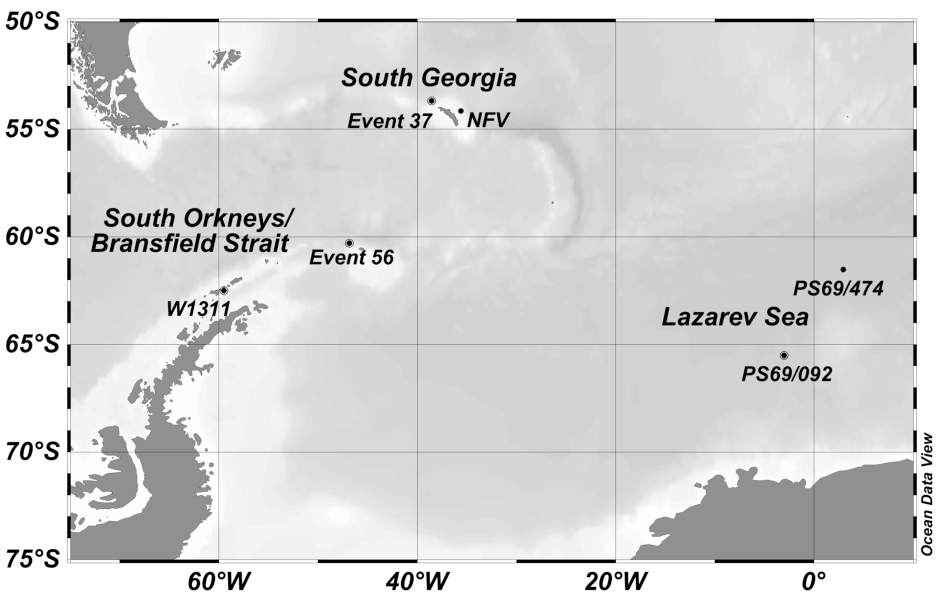
\includegraphics[width=0.85\textwidth]{../Figures/Pub1_1.pdf} 
        \caption{Station map indicating station numbers (NFV - Norwegian fishing vessel) and the three
studied regions} 
        \label{Pub1_1} 
\end{figure}

\section{Methods}

\subsection{Sample collection and experimental design}

Antarctic krill samples (\textit{Euphausia superba}) were obtained from five
different expeditions and from a Norwegian fishing vessel (Table \ref{Tab1_1},
Fig. \ref{Pub1_1}.  Sampling was carried out with a Rectangular Midwater Trawl
(RMT8+1 for expeditions ANT23-2, ANT23-6 and JR15004, RMT8 for expedition
JR260B), an Isaacs-Kidd Midwater Trawl (IKMT, expedition AMLR14) and a
continuous pumping system (Norwegian fishing vessel). Snap-frozen Antarctic
krill samples stored at \SI{-80}{\celsius} were transferred to the
Alfred-Wegener-Institute, Bremerhaven, for molecular analysis.


% Table I Please add the following required packages to your document preamble:
% \usepackage[normalem]{ulem} \useunder{\uline}{\ul}{}
\begin{table}[] {\scriptsize \caption{Sampling data including cruise, region,
        station, sampling date
        and local time (h:min), season, latitude, longitude, sampling gear,
        number of individuals with sex, and sample code of the analysed
        individuals}
        \begin{tabular}{@{}L{1.75cm}L{1cm}lllllL{1.5cm}l@{}}
\toprule
\textbf{Cruise} & \textbf{Region} & \textbf{Station} & \textbf{Date/Time} & \textbf{Season} & \textbf{Latitude} & \textbf{Longitude} & \textbf{Gear} & \textbf{Sex} \\
\midrule
ANT23-2                  & Lazarev Sea       & PS69/092 & 23. Dec 05 & summer & -65.51   & -3.03     & RMT 8+1                   & 3 \male \\
                         &                   &          & 01:07      &        &          &           &                           & 4 \female \\
ANT23-6                  & Lazarev Sea       & PS69/474 & 27. Jun 06 & winter & -61.52   & 2.93      & RMT 8+1                   & 3 \male \\
                         &                   &          & 02:21      &        &          &           &                           & 3 \female \\
JR15004                  & South Orkneys     & Event 56 & 02. Feb 16 & summer & -60.30   & -46.85    & RMT8+1                    & 3 \male \\
                         &                   &          & 04:14      &        &          &           &                           & 3 \female \\
AMLR14                   & Bransfield Strait & W1311    & 26. Aug 14 & winter & -62.50   & -59.50    & IKMT                      & 3 \male \\
                         &                   &          & 00:40      &        &          &           &                           & 3 \female \\
JR260B                   & South Georgia     & Event 37 & 04. Jan 12 & summer & -53.68   & -38.56    & RMT 8                     & 3 \male \\
                         &                   &          & 01:37      &        &          &           &                           & 3 \female \\
Norwegian fishing vessel & South Georgia     &          & 18. Jul 15 & winter & -54.15   & -35.60    & continuous pumping system & 5 \male \\
                         &                   &          & 07:00      &        &          &           &                           & \\
\bottomrule
\end{tabular}
        \label{Tab1_1}
        }
\end{table}

The Antarctic krill originated from three different latitudinal regions: a)
Lazarev Sea (\SI{62}{\degree}S-\SI{66}{\degree}S), b) South Orkneys/Bransfield
Strait (\SI{60}{\degree}S-\SI{63}{\degree}S), and c) South Georgia
(\SI{54}{\degree}S), including summer and winter samples for each region.  By
visual inspection of the outer sexual organs, male petasma and female thelycum,
adult males and females were identified. In total, 36 individuals were chosen
for further analysis, with 6-7 individuals for each regional and seasonal
sample including 3-4 females and 3 males (except the South Georgia winter
sample, where solely males were available, and 5 males were analysed; see Table
\ref{Tab1_1} for full sampling scheme).

\subsection{RNA extraction, library preparation and Illumina sequencing}

RNA extraction was performed from frozen krill heads with the RNeasy Midi Kit
(QIAGEN, Hilden, Germany). Frozen krill heads were cut on dry ice and
transferred to \SI{1.5}{\milli\litre} RLT lysis buffer in tissue homogenizing
Precellys\textsuperscript{\textregistered} tubes (CKMix Tissue Homogenizing
Kit, Bertin corp., Rockville, MD, USA).  Homogenization was carried out at
\SI{4}{\celsius} in a Precellys\textsuperscript{\textregistered} homogenizer
with the Cryolys\textsuperscript{\textregistered} cooling system (Bertin corp.)
with two runs for \SI{15}{\second} at 5000 rpm and \SI{10}{\second} break.
Further steps of RNA extraction were carried out according to the
manufacturer's protocol of the RNeasy Midi Kit. The quality and quantity of the
RNA was inspected using the NanoDrop\texttrademark 2000 UV-Vis
Spectrophotometer (Thermo Fisher Scientific, Waltham, MA, USA) and the Agilent
2100 Bioanalyzer system (Agilent technologies, Santa Clara, CA, USA).

RNA samples were sent for sequencing to IGA Technology Services (Udine, Italy).
cDNA libraries were performed with \SIrange{1}{2}{\micro\gram} RNA by using the
TruSeq Stranded mRNA Sample Prep kit (Illumina, San Diego, CA, USA) following
the manufacturer's instructions. The poly-A mRNA was fragmented 3 minutes at
\SI{94}{\celsius}. 1X Agencourt AMPure XP beads (Agencourt Bioscience
Cooperation, Beckman Coulter, Beverly, MA, USA) were used for every
purification step. The RNA samples and final cDNA libraries were quantified
with the Qubit 2.0 Fluorometer (Invitrogen, Carlsbad, CA, USA) and quality
tested by Agilent 2100 Bioanalyzer Nano assay.  For cluster generation on the
flow cell, libraries were processed with cBot (Illumina, San Diego, CA, USA)
following manufacturer's instructions.  Sequencing was carried out on
paired-end mode (2 $\times$ 100 bp) on HiSeq2500 (Illumina) with a targeted
sequencing depth of about 80 million reads per sample. Raw data were processed
with the software \code{CASAVA v1.8.2} (Illumina) for both format conversion
and de-multiplexing.

\subsection{Quality control and analysis of RNA-seq data}

The programme \code{BBDuk} from \code{BBMap package v36.38}
\citep{bushnell_bbmap._2016} was used for the removal of adapter sequences and
quality trimming of reads (set parameters: ktrim=r, k=23, mink=11, hdist=1, tpe
tbo, qtrim=r, trimq=10, minlen=36). The quality of the trimmed reads was
checked with the programme \code{FastQC v0.11.5} \citep{andrews_fastqc:_2017}.
Since the \code{FastQC} reports indicated the presence of reads encoding
ribosomal RNA, these reads were removed using the software \code{SortMeRNA
v2.1} \citep{kopylova_sortmerna:_2012}.  Transcript abundance in each sample
was estimated by aligning the processed paired-end reads to the \textit{E.
superba} reference transcriptome \citep{meyer_pyrosequencing_2015} using the
software \code{Trinity v2.4.0} \citep{grabherr_full-length_2011} with the
abundance estimation method \code{RSEM v1.2.26} \citep{li_rsem:_2011} and the
alignment tool \code{Bowtie2 v2.2.5} \citep{langmead_fast_2012}. As reference,
we chose the transcriptome by \citet{meyer_pyrosequencing_2015} instead of the
recently developed KrillDB transcriptome \citep{sales_krilldb:_2017}, because
preliminary alignment tests yielded approximately 10\% higher alignment rates
to the transcriptome by \citet{meyer_pyrosequencing_2015}. Both transcript
expression matrix of non-normalized counts and matrix of TMM-normalized
expression values were calculated. Mapping rates to the reference transcriptome
had a mean $\pm$ SD of $69.22 \pm 3.37$\%. Differential gene expression was
analysed with \code{edgeR} \citep{robinson_edger:_2010}. Significant
differentially expressed genes (DEGs) were identified using a false discovery
rate (FDR) cutoff value of $0.001$ and a minimum absolute Log2 fold change
(log2FC) of 2. Pairwise comparisons included seasonal comparisons within each
region and regional comparisons in both summer and winter between regions (Fig.
\ref{Pub1_2}). The PtR script was used to do a principal component analysis
(PCA) of all differentially expressed transcripts.  Both PC 1 and PC 2 were
correlated to season accounting for overall 46.89\% variation in the dataset
(supplementary Figure S1), but did not show correlation to region, sex or
sample processing.

% Figure 2
\begin{figure} 
        \centering
        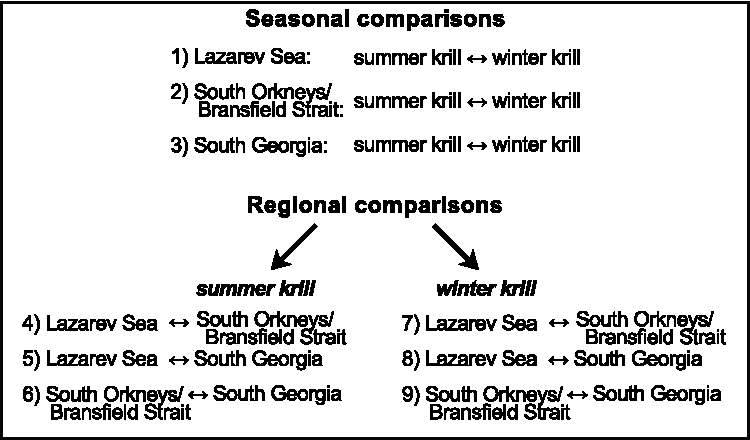
\includegraphics[width=0.85\textwidth]{../Figures/Pub1_2.pdf}
        \caption{Pairwise comparisons tested for differentially
        expressed transcripts subdivided into seasonal comparisons between
        summer and winter in three different regions (1-3) and regional
        comparisons of summer krill (4-6) and winter krill (7-9).}
        \label{Pub1_2}
\end{figure}

To annotate the DEGs, local blastx searches against the protein UniProt
databases Swiss-Prot and UniRef90 \citep{boutet_uniprotkb/swiss-prot_2007} with
a cutoff E value of $10^{-9}$ were performed using \code{BLAST+ v.2.5.0}
\citep{camacho_blast+:_2009}.  From the 1929 DEGs, 693 genes could be annotated
resulting in an annotation rate of 35.93\%. Additional annotation information
were retrieved from the UniProt website (\url{https://www.uniprot.org/}). To
aim for a crustacean-specific annotation and functional characterization, we
chose to do a manual categorization of the annotated genes rather than
focussing on the enrichment of gene ontology (GO) terms. Thereby, we were also
able to improve the functional characterization of DEGs for the regional and
seasonal comparisons where only few DEGs were found (Table \ref{Tab1_2}). Using
the information from the UniProt website and crustacean-specific literature, if
available, the annotated genes were inspected and sorted manually into
categories (supplementary Table S1). For selected genes of interest, the
annotation was reviewed performing blastx searches against NR using the web
interface on \url{https://blast.ncbi.nlm.nih.gov/Blast.cgi}  (Johnson et al.,
2008). For contigs HACF01031034, HACF01033533, HACF01010344 and HACF01005894,
improved annotation results were added to the annotation table (supplementary
Table S1).  For Fig. \ref{Pub1_3} and supplementary Figure S2 , category
normalization was carried out by dividing the DEG counts per category for
upregulated genes per sample by the size of the respective category (total
count of DEGs within the same category).  Normalized categories are shown in
normalized units ranging from 0 to 1 indicating a higher importance of
categories with increasing values towards 1.  Top categories were defined for
values higher or equal to 0.2.

% Table 2
% Table II

% Please add the following required packages to your document preamble:
% \usepackage{booktabs}
\begin{table}[]
{\scriptsize
\caption{Number of differentially expressed transcripts (DETs) identified for each tested pairwise comparison in edgeR including the number of upregulated DETs in each sample}
\label{Tab1_2}
\begin{tabular}{@{}llllL{1.5cm}L{1.5cm}@{}}
\toprule
\textbf{Test} & \textbf{Sample A}         & \textbf{Sample B}         & \textbf{Total no. of DETs} & \textbf{Upregulated in sample A} & \textbf{Upregulated in Sample B} \\ \midrule
1             & Lazarev Sea, summer       & Lazarev Sea, winter       & 698                        & 611                              & 87                               \\
2             & South Orkneys, summer     & Bransfield Strait, winter & 1121                       & 1054                             & 67                               \\
3             & South Georgia, summer     & South Georgia, winter     & 295                        & 251                              & 44                               \\
4             & Lazarev Sea, summer       & South Orkneys, summer     & 234                        & 143                              & 91                               \\
5             & Lazarev Sea, summer       & South Georgia, summer     & 132                        & 69                               & 63                               \\
6             & South Orkneys, summer     & South Georgia, summer     & 82                         & 64                               & 18                               \\
7             & Lazarev Sea, winter       & Bransfield Strait, winter & 73                         & 37                               & 36                               \\
8             & Lazarev Sea, winter       & South Georgia, winter     & 174                        & 24                               & 150                              \\
9             & Bransfield Strait, winter & South Georgia, winter     & 106                        & 73                               & 33                               \\ \bottomrule
\end{tabular}
}
\end{table}


% Figure 3
\begin{figure} 
        \centering
        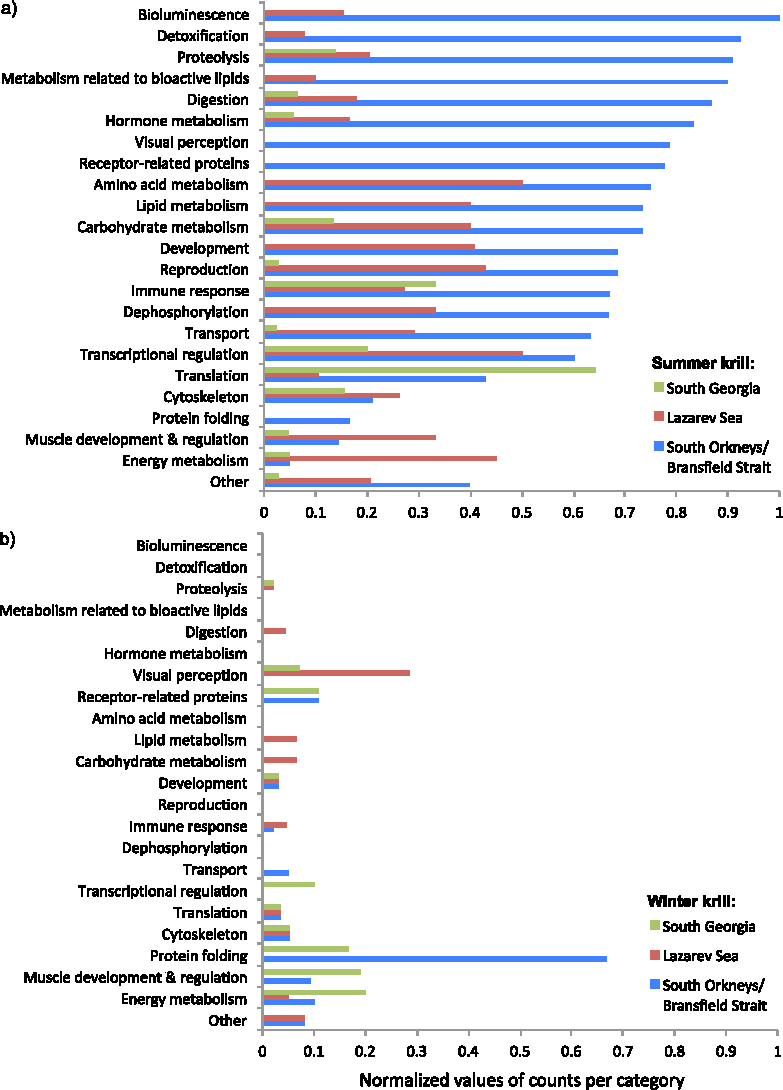
\includegraphics[width=0.85\textwidth]{../Figures/Pub1_3.pdf}
        \caption{Bar plots showing the functional categories found in the three
        seasonal comparisons with a) normalized category values of upregulated
        differentially expressed genes in summer krill from each region, and b)
        normalized category values of upregulated differentially expressed
        genes in winter krill from each region.}
        \label{Pub1_3}
\end{figure}
\subsection{Data archiving}

Raw sequences and the transcript expression matrix of non-normalized counts
have been deposited in the ArrayExpress database at \texttt{EMBL-EBI}
(\url{www.ebi.ac.uk/arrayexpress}) under accession number \texttt{E-MTAB-7467}.

\section{Results}

\subsection{Seasonal comparisons of gene expression in three different latitudinal regions}

Highest differential gene expression was found in the seasonal pairwise
comparisons in the three regions with 295 to 1121 DEGs which were mostly
upregulated in summer krill (Table \ref{Tab1_2}). Most DEGs were found in the
winter-summer krill comparison of the South Orkneys/Bransfield Strait region,
followed by Lazarev Sea and South Georgia. Krill from the South Georgia region
had the lowest seasonal differences in gene expression compared to the other
regions.

The highest functional variety of DEGs was found to be upregulated in summer
krill from the South Orkneys/Bransfield Strait region (Fig. \ref{Pub1_3}a). The
19 top categories comprised bioluminescence (1), detoxification (0.92),
proteolysis (0.91), metabolism related to bioactive lipids (0.9), digestion
(0.87), hormone metabolism (0.83), visual perception (0.79),  receptor-related
proteins (0.78), amino acid metabolism (0.75), carbohydrate and lipid
metabolism (0.74 each), development and reproduction (0.69 each), immune
response and dephosphorylation (0.67 each), transport (0.63), transcriptional
regulation (0.6), translation (0.43) and cytoskeleton (0.21). Thereof, the
first 8 categories were particularly distinct for South Orkneys/Bransfield
Strait summer krill with respect to the other two studied regions.

For Lazarev Sea summer krill, 13 top categories were found: amino acid
metabolism and transcriptional regulation (0.5 each), energy metabolism (0.45),
reproduction (0.43), development (0.41), carbohydrate and lipid metabolism (0.4
each), muscle development \& regulation and dephosphorylation (0.33 each),
transport (0.29), immune response (0.27), cytoskeleton (0.26) and proteolysis
(0.2). Compared to summer krill from the other two studied  regions, the
categories energy metabolism and muscle development \& regulation had highest
values in Lazarev Sea summer krill. 

For South Georgia summer krill, only three top categories were identified:
translation (0.64), immune response (0.33) and transcriptional regulation
(0.2). Compared to the other two regions, the category translation was most
pronounced in South Georgia summer krill. Most genes related to other
metabolic, regulatory and biological processes were not differentially
expressed in South Georgia krill.

Compared to summer krill, only few DEGs were found to be upregulated in winter
krill from the three regions (Fig. \ref{Pub1_3}b).  Only one top category was
found for winter krill from each studied region: protein folding (0.67) for
South Orkneys/Bransfield Strait, visual perception (0.29) for Lazarev Sea, and
energy metabolism (0.2) for South Georgia. 

Detailed \code{edgeR} results of the seasonal differential expression analysis
can be found in the supplementary Table SII.

\subsection{Detailed analysis of categories including genes with putative seasonal regulatory functions}

With the aim to look for target genes with potential seasonal regulatory
functions in Antarctic krill, we chose the following 7 categories for further
investigation: metabolism related to bioactive lipids, hormone metabolism,
visual perception, receptor-related proteins, development, reproduction,
dephosphorylation and transcriptional regulation. The analysis was not
restricted to the samples where these categories were enriched, but all
identified DEGs within these categories were inspected. Selected members of
these categories are shown in Table \ref{Tab1_3}. 

% Please add the following required packages to your document preamble:
% \usepackage{booktabs}
% \usepackage{longtable}
% Note: It may be necessary to compile the document several times to get a multi-page table to line up properly
%\begin{landscape}
{\scriptsize
\begin{longtable}{@{}L{1.8cm}L{3cm}L{2cm}L{2.5cm}L{1.75cm}L{2.5cm}@{}}
\caption{Selected members of differentially expressed protein-coding genes of
        the seasonal comparisons within the categories metabolism related to
        bioactive lipids, hormone metabolism, visual perception,
        receptor-related proteins, development, reproduction, dephosphorylation
        and transcriptional regulation}
\label{Tab1_3}\\
\toprule
\textbf{Category}                      & \textbf{Protein}                                                        & \textbf{Related Swissprot / UniRef / NR ID} & \textbf{Putative function}                                                                           & \textbf{Contig ID} & \textbf{Upregulated in}              \\* \midrule
\endfirsthead
%
\multicolumn{6}{c}%
{{\bfseries Table \thetable\ continued from previous page}} \\
\toprule
\textbf{Category}                      & \textbf{Protein}                                                        & \textbf{Related Swissprot/UniRef/NR ID} & \textbf{Putative function}                                                                           & \textbf{Contig ID} & \textbf{Upregulated in}              \\* \midrule
\endhead
%
\bottomrule
\endfoot
%
\endlastfoot
%
Metabolism related to bioactive lipids & Sphingomyelin phosphodiesterase                                         & Q0VD19                                  & sphingolipid metabolism, biosynthesis of ceramide                                                    & HACF01033273       & South Orkneys, summer                \\
                                       & Putative glucosylceramidase 4                                           & Q9UB00                                  & sphingolipid metabolism, biosynthesis of ceramide                                                    & HACF01006732       & South Orkneys, summer                \\
                                       & Neutral ceramidase                                                      & Q29C43                                  & sphingolipid metabolism, biosynthesis of sphingosine                                                 & HACF01032702       & South Orkneys, summer                \\* \midrule
Hormone metabolism                     & Dehydrogenase/reductase SDR family member 11                            & Q71R50                                  & estrogen biosynthesis                                                                                & HACF01041540       & South Orkneys, summer                \\
                                       & Lathosterol oxidase                                                     & Q9EQS5                                  & steroid metabolism                                                                                   & HACF01002294       & South Orkneys, summer                \\
                                       & Cytochrome P450 3A21                                                    & O18993                                  & steroid metabolism                                                                                   & HACF01007387       & South Orkneys, summer                \\
                                       & Type I iodothyronine deiodinase                                         & P24389                                  & thyroxine metabolism                                                                                 & HACF01008075       & South Orkneys, summer                \\
                                       & Beta,beta-carotene 9',10'-oxygenase                                     & Q99NF1                                  & retinoic acid biosynthesis                                                                           & HACF01008355       & South Orkneys, summer                \\
                                       & Aldehyde dehydrogenase family 8 member A1                               & Q9H2A2                                  & retinoic acid biosynthesis                                                                           & HACF01003376       & Lazarev Sea, summer                  \\
                                       & Tyrosine decarboxylase                                                  & Q95ZS2                                  & octopamine biosynthesis                                                                              & HACF01001558       & Lazarev Sea, summer                  \\
                                       & Neprilysin-1                                                            & W4VS99                                  & breakdown of neuropeptides                                                                           & HACF01002648       & South Orkneys, summer                \\
                                       & Neuroendrocrine convertase 1                                            & OAD61081.1                              & cleavage of precursors of bioactive peptides                                                         & HACF01005894       & South Orkneys, summer                \\* \midrule
Visual perception                      & Arrestin homolog                                                        & P55274                                  & signal transduction                                                                                  & HACF01056943       & South Orkneys, summer                \\
                                       & Arrestin, lateral eye                                                   & P51484                                  & signal transduction                                                                                  & HACF01005913       & Lazarev Sea, winter                  \\
                                       & Carotenoid isomerooxygenase                                             & Q9VFS2                                  & visual pigment biogenesis, photoreceptor development                                                 & HACF01003645       & South Orkneys, summer                \\* \midrule
Receptor-related proteins              & Adiponectin receptor protein                                            & Q9VCY8                                  & regulation of insulin secretion, glucose and lipid metabolism                                        & HACF01002955       & South Orkneys, summer                \\
                                       & Prolow-density lipoprotein receptor-related protein 1                   & Q07954                                  & multiple functions in development, cellular lipid homeostasis, signalling and neurotransmission      & HACF01040030       & South Orkneys, summer                \\
                                       & Leucine-rich repeat-containing G-protein coupled receptor 4             & A2ARI4                                  & activator of Wnt signalling pathway, development, regulation of circadian rhythms of plasma lipids   & HACF01008235       & South Orkneys, summer                \\
                                       & Integrin beta-1-A                                                       & P12606                                  & formation of receptor complexes with wide array of ligands                                           & HACF01056144       & South Orkneys, summer                \\
                                       & Translocon-associated protein subunit gamma                             & Q9DCF9                                  & regulation of retention of ER resident proteins                                                      & HACF01039823       & Bransfield Strait, winter            \\
                                       & Guanine nucleotide-binding protein subunit beta-2-like 1                & O42248                                  & recruitment, assembly and regulation of various signalling molecules                                 & HACF01000518       & South Georgia, winter                \\* \midrule
Development                            & Blastula protease 10                                                    & P42674                                  & cell differentiation                                                                                 & HACF01031830       & South Orkneys, Lazarev Sea, summer   \\
                                       & Protein SpAN                                                            & P98068                                  & cell differentiation                                                                                 & HACF01012692       & Lazarev Sea, winter                  \\
                                       &                                                                         &                                         &                                                                                                      &                    &                                      \\
                                       & Carbohydrate sulfotransferase 11                                        & Q9NPF2                                  & regulation of cell proliferation                                                                     & HACF01012160       & South Orkneys, Lazarev Sea, summer   \\
                                       & Fibrocystin-L                                                           & Q80ZA4                                  & regulation of cell proliferation                                                                     & HACF01005119       & South Orkneys, Lazarev Sea, summer   \\
                                       & Glycoprotein 3-alpha-L-fucosyltransferase A                             & Q9VUL9                                  & nervous system development                                                                           & HACF01046985       & South Orkneys, summer                \\
                                       & Neurotrophin 1                                                          & B7TB45                                  & nervous system development                                                                           & HACF01037993       & Lazarev Sea, summer                  \\
                                       & Laccase-2 isoform X4                                                    & XP\_025270057.1                         & cuticle tanning                                                                                      & HACF01010344       & South Orkneys, Lazarev Sea, summer   \\
                                       & Crustacyanin-A2 subunit                                                 & P80007                                  & coloration                                                                                           & HACF01009046       & Bransfield Strait, winter            \\
                                       &                                                                         &                                         &                                                                                                      &                    &                                      \\
                                       & Krueppel homolog 1                                                      & P08155                                  & metamorphosis                                                                                        & HACF01005245       & South Georgia, winter                \\* \midrule
Reproduction                           & Vitellogenin                                                            & Q6RG02                                  & lipid transport, oogenesis                                                                           & HACF01038168       & South Orkneys, Lazarev Sea, summer   \\
                                       & Vitellogenin 2                                                          & UniRef90\_V9XZL5                        & lipid transport, oogenesis                                                                           & HACF01038626       & South Orkneys, South Georgia, summer \\
                                       & Hematopoietic prostaglandin D synthase                                  & O73888                                  & prostaglandin biosynthesis                                                                           & HACF01038076       & South Orkneys, Lazarev Sea, summer   \\
                                       & Prostamide/prostaglandin F synthase                                     & Q8TBF2                                  & prostaglandin biosynthesis                                                                           & HACF01001735       & South Orkneys, summer                \\
                                       & Carbonyl reductase {[}NADPH{]} 1                                        & P48758                                  & prostaglandin biosynthesis                                                                           & HACF01007962       & South Orkneys, summer                \\
                                       & Juvenile hormone esterase-like protein 1                                & ALT10383.1                              & potential role  in degradation of methyl farnesoate                                                  & HACF01031034       & South Orkneys, summer                \\
                                       & Juvenile hormone esterase-like carboxylesterase 1                       & APO14259.1                              & potential role  in degradation of methyl farnesoate                                                  & HACF01033533       & Lazarev Sea, summer                  \\* \midrule
Dephosphorylation                      & Serine/threonine-protein phosphatase 2A catalytic subunit alpha isoform & P48463                                  & modulation of phosphorylase B kinase casein kinase 2, mitogen-stimulated S6 kinase, and MAP-2 kinase & HACF01002873       & Lazarev Sea, summer                  \\* \midrule
Transcriptional regulation             & CREB-binding protein                                                    & P45481                                  & transcriptional regulation                                                                           & HACF01024140       & Lazarev Sea, summer                  \\* \bottomrule
\end{longtable}
%\end{landscape}
}


Genes within the category metabolism related to bioactive lipids were enriched
in the South Orkneys/Bransfield Strait summer krill. Some of these genes were
also found in Lazarev Sea summer krill. These genes had predicted functions in
sphingolipid metabolism, such as the biosynthesis of ceramide and sphingosine,
and in the biosynthesis of phosphatidylcholine.

The category hormone metabolism was found to be enriched in the South
Ork\-neys/Brans\-field strait summer krill. However, few genes within this category
were also upregulated in summer krill from the other two regions. Genes within
category hormone metabolism had predicted functions in steroid metabolism,
thyroxine metabolism, retinoic acid biosynthesis, octopamine biosynthesis,
taurine biosynthesis and the breakdown of bioactive peptides.

Genes within the category visual perception were enriched and upregulated in
the South Orkneys/Bransfield Strait summer krill and in Lazarev Sea winter
krill. This category comprised genes related to signal transduction, visual
pigment biogenesis and eye development.

The category receptor-related proteins was enriched in the South
Ork\-neys/Brans\-field Strait summer krill. Two genes of this category were also
found to be upregulated in the South Orkneys/Bransfield Strait and South
Georgia winter krill. These genes coded for different receptor-related proteins
with predicted functions in the formation of receptor complexes and various
signalling pathways and regulatory processes, such as the Wnt and insulin
signalling pathway.

The category development was found to be enriched in South Orkneys/Bransfield
Strait and Lazarev Sea summer krill. Three genes of this category were
upregulated in the winter krill of the three studied regions. The genes had
predicted functions in cell differentiation and proliferation, nervous system
development, pigmentation, metamorphosis and the regulation of other
development processes.

The category reproduction was enriched in South Orkneys/Bransfield Strait and
Lazarev Sea summer krill. A few DEGs within this category were also upregulated
in South Georgia summer krill. This category included DEGs with putative
functions as the lipid transporter vitellogenin and in the metabolism of
reproduction-related hormones, in particular prostaglandin biosynthesis and
juvenile hormone esterase-like carboxyesterases.

The category dephosphorylation contained only three DEGs which coded for
putative phosphatases. The category was enriched in South Orkneys/Bransfield
Strait and Lazarev Sea summer krill.

The category transcriptional regulation was found to be enriched in summer
krill of the three studied regions. One gene within this category was
identified in South Georgia winter krill. These DEGs coded for proteins with
putative RNA binding activity and regulatory functions in transcription.

\subsection{Regional comparisons of gene expression within each season (summer and winter)}

Less genes were differentially expressed in the regional pairwise comparisons
in summer (82 to 234 DEGs) and winter (73 to 174 DEGs) (Table \ref{Tab1_2}). A
plot showing the results of the regional comparisons can be found in the
supplementary material (Fig. S2).

Comparing the three regional summer samples from South Orkneys/Bransfield
Strait, Lazarev Sea and South Georgia, least DEGs were found within the
comparison South Orkneys/Bransfield Strait vs. South Georgia krill. Only few
upregulated DEGs from the South Orkneys/Bransfield Strait latitudinal region
could be annotated compared to the other regions in summer. In the South
Orkneys/Bransfield Strait summer krill the category visual perception was
enriched with respect to Lazarev Sea and South Georgia summer krill (0.21
each). Lazarev Sea summer krill showed two enriched top categories with respect
to South Orkneys/Bransfield Strait summer krill only: energy metabolism (0.25)
and reproduction (0.26) comprising vitellogenin-like genes only. South Georgia
summer krill had two top categories with respect to Lazarev Sea summer krill
only: cytoskeleton (0.32) and translation (0.68).

Comparing the three regional winter samples, only few DEGs could be annotated.
The category  carbohydrate metabolism (0.2) was found to be enriched for the
South Georgia winter krill with respect to Lazarev Sea winter krill only. 

Detailed \code{edgeR} results of the regional differential expression analysis
can be found in the supplementary Table SIII.

\section{Discussion}

\subsection{Generalisations and methodological discussion}

This study investigated seasonal and regional differences in gene expression in
Antarctic krill in three different latitudinal regions of the Southern Ocean
(Lazarev Sea: 62$^{\circ}$S-66$^{\circ}$S, South Orkneys/Bransfield Strait:
60$^{\circ}$S-63$^{\circ}$S, and South Georgia: 54$^{\circ}$S). Seasonal
differences between summer and winter krill were generally found to be more
pronounced than regional differences in summer or winter. Most differentially
expressed genes were found to be upregulated in summer krill indicating that
Antarctic krill entered a less active state during winter in all studied
regions. However, these seasonal differences in gene expression seemed to be
less distinct in the low-latitude region South Georgia.

Differences in the seasonal gene expression pattern between the three tested
regions may reflect an adaptive behaviour of Antarctic krill to the
environmental conditions that krill is exposed to in the different habitats.
The highest variety of functionally enriched genes was found in the South
Orkneys/Bransfield Strait region which indicates that summer krill was in a
highly active condition in this region with respect to winter. In particular,
Antarctic summer krill from South Orkneys/Bransfield Strait were characterized
by the upregulation of genes related to bioluminescence, detoxification,
metabolism related to bioactive lipids, digestion, hormone metabolism, visual
perception and receptor-related proteins. The upregulation of amino acid, lipid
and carbohydrate metabolism and the biological categories reproduction and
development in both South Orkneys/Bransfield Strait and Lazarev Sea summer
krill with respect to winter supports the assumption that krill enters a state
of metabolic depression and regressed development during winter in these
regions (so called winter quiescence). However, genes related to energy
metabolism were found to be upregulated in Lazarev Sea summer krill only. This
may point to stronger seasonal differences in energy metabolism in the
high-latitude region Lazarev Sea. In contrast, most genes related to metabolic,
biological and regulatory processes were not found to be differentially
expressed in the comparison of summer and winter krill from South Georgia which
may be a response to the less extreme winter conditions in this low-latitude
region \citep{meyer_winter_2017}.

We also identified a variety of candidate genes with likely roles in the
metabolism related to bioactive lipids, hormone metabolism, visual perception,
as receptor-related proteins, in development, reproduction, dephosphorylation
and transcriptional regulation. The selected genes may serve as target genes
for future studies of seasonal rhythms in Antarctic krill.

This paper partly confirms results from a microarray study by
\citet{seear_seasonal_2012} who found an upregulation of genes involved in
feeding and digestion, respiration, motor activity, immunity and vitellogenesis
in Antarctic krill near the Antarctic Peninsula (60$^{\circ}$S) in summer. By
contrast, the present paper investigated as novel aspect the seasonal gene
expression profiles of Antarctic krill from three different latitudinal regions
in the Atlantic sector of the Southern Ocean. In particular, it adds seasonal
gene expression data for summer and winter krill from the high-latitude region
Lazarev Sea and the low-latitude region South Georgia. Moreover, the present
study used a different molecular approach, RNA-seq, focussing on putative
regulatory processes of seasonal rhythms in Antarctic krill and the
identification of potential seasonal target genes. In contrast to the study by
\citet{seear_seasonal_2012}, we did not find strong differences in the direct
regional comparisons of the summer or winter krill samples, such as the
upregulation of genes related to digestion and immunity in the South Georgia
region in winter \citep{seear_seasonal_2012}.  Moreover, we observed a more
diverse pattern of gene expression related to energy metabolism and respiration
in the three studied regions.

These differences may have been caused by different methodological constraints
of our RNAseq study. A limited number of Antarctic krill samples were available
for sequencing. The sequenced Antarctic krill originated from the field and
were sampled under highly variable conditions. Social cues, feeding condition,
migratory behaviour of krill, and abiotic factors that cannot be controlled may
have affected the gene expression profile detected in the samples. Moreover,
differences in sampling time and station coordinates, variable sampling
techniques on the different vessels and unknown parameters such as age or
moulting stage of the studied individuals may have introduced variation in the
dataset. To partly compensate for this variation, we used high replicate
numbers for differential gene expression analysis in this RNAseq study.

In this study, the generally low level of upregulated genes in winter krill
cannot directly explain the winter behaviour of Antarctic krill in some
regions. For instance, the Bransfield Strait is a food-rich overwintering
ground for Antarctic krill where large vertical migrations have been observed
\citep{bernard_contribution_2018, reiss_overwinter_2017}. Hence, gene
expression needs to be activated in winter to allow for this behaviour.
However, our data analysis focussed on significant differences in seasonal gene
expression. It mainly revealed genes that are important for Antarctic krill in
its more active summer condition, where gene expression is apparently much
larger with respect to winter. But the expression of genes below the detection
level of our statistical methods may still allow for winter feeding and
migration behaviour.

\subsection{Potential influences on Antarctic krill's seasonal and regional gene expression}

Our seasonal  gene expression results from South Orkneys/Bransfield Strait and
Lazarev Sea agree with observations in Antarctic krill from the field: a
reduced metabolic activity and regressed development in winter and an enhanced
metabolism, development, reproductive activity and gene expression in summer
\citep{meyer_seasonal_2010, siegel_krill_2012}. In contrast, metabolic
depression in winter and enhanced expression of reproduction- and development
related genes in summer were not observed in the South Georgia krill.  Yet,
generally higher gene expression was also found in the South Georgia summer
krill related to other processes such as translation, immune response and
transcriptional regulation. These differences in seasonal gene expression
discovered in krill from the South Georgia region may reflect the flexible
overwintering behaviour of Antarctic krill found in this region
\citep{schmidt_feeding_2014}.

Variable factors such as water temperature, reproductive timing, food
availability and light regime may have influenced the regional differences
observed in seasonal gene expression in Antarctic krill in this study.

However, regional differences in seasonal water temperature cannot explain why
the least seasonal differences in gene expression were found in the South
Georgia region. Largest seasonal differences in water temperature are observed
around South Georgia, where temperature may rise above 4$^{\circ}$C in summer
and remains around 0$^{\circ}$C in winter \citep{whitehouse_seasonal_1996}. In
contrast, seasonal water temperatures are more stable in the Lazarev Sea and
close to the Antarctic Peninsula ranging between -1.8$^{\circ}$C  and
-0.1$^{\circ}$C (\citet{meyer_seasonal_2010}, and station data), but krill from
these regions showed the largest differences in seasonal gene expression in our
study.

The variable reproductive timing of Antarctic krill according to region and sea
ice conditions \citep{spiridonov_spatial_1995} may explain why in our study
less seasonal differences in gene expression were observed in the Lazarev Sea
compared to South Orkneys/Bransfield Strait. Summer krill samples from Lazarev
Sea were obtained in the end of December, when sea ice was melting and the
phytoplankton bloom just started to develop \citep{meyer_seasonal_2010}. Thus,
the krill from the Lazarev Sea was probably only in preparation of the spawning
season. On the contrary, the South Orkneys/Bransfield Strait krill was caught
in an ice-free region in the beginning of February, where krill was in the
middle of the spawning period and probably in a more active condition than in
Lazarev Sea.  The high metabolic demand of the South Orkneys/Bransfield Strait
summer krill is reflected by the high proportion of detoxification genes found
in this region.

Annual feeding conditions may have especially affected the different behaviour
of Antarctic krill in the lower-latitudinal region South Georgia, where krill
is exposed to less extreme winter conditions compared to the other two regions.
South Georgia is ice-free throughout the year and prolonged periods of
phytoplankton blooms occur in this area. In winter, Antarctic krill from South
Georgia was observed to be feeding on phytoplankton and seabed detritus, and
contained lower lipid stores compared to Antarctic krill from Bransfield Strait
and Lazarev Sea \citep{schmidt_feeding_2014}. Therefore, seasonal differences
in gene expression may be less pronounced in that area.

There are indications that light regime and an endogenous timing system may
play a major role in controlling the flexible behaviour and life cycle of
Antarctic krill in different latitudinal regions of the Southern Ocean.
Recently, a two-year lab experiment has shown that the latitudinal light regime
(photoperiod, the day length) affected seasonal cycles of growth, maturity,
feeding and lipid content of Antarctic krill \citep{horing_light_2018}.
Seasonal patterns of growth, feeding and maturity were also observed under
constant darkness which indicated the presence of an endogenous timing system
that was most likely entrained by light regime prior to the experiments.
Critical photoperiods for female maturity were found to be higher under the
simulated high-latitude light regime which pointed to a flexible seasonal
timing system in Antarctic krill under different latitudinal photoperiods.
\citet{piccolin_seasonal_2018} demonstrated the effect of photoperiod on the
seasonal cycle of growth, enzyme activity and oxygen consumption in Antarctic
krill. The authors linked the results to the seasonal expression of circadian
clock genes and suggested their involvement in the seasonal timing mechanism in
Antarctic krill.

These findings reveal that photoperiod is an important zeitgeber for Antarctic
krill that seems to entrain its seasonal timing system under the variable
photoperiodic conditions in the Southern Ocean. The less pronounced seasonal
cycle of Antarctic krill observed around South Georgia may therefore be partly
controlled by the less extreme seasonal light conditions in that region and
krill's endogenous clock. The photoperiodic seasonal timing system may be
complemented by other factors such as food supply as explained above.

\subsection{Target genes and their putative functions in Antarctic krill}

We identified regulatory genes with multiple functions that may play an
important role in the control of seasonal physiology and behaviour in Antarctic
krill. These target genes were selected from annotated genes with putative
regulatory functions that were differentially expressed between summer and
winter krill in this study. The functional roles of these genes still need to
be validated in Antarctic krill in future laboratory experiments. Moreover,
controlled laboratory experiments may be conducted to test if these genes are
rhythmically expressed under different light regimes and if they are
effectively involved in the regulation of seasonal life cycle events in
Antarctic krill. Thus, our study establishes a basis for future laboratory
studies to further elucidate the molecular mechanisms of seasonal rhythms in
Antarctic krill. In the following, we will describe the potential functional
roles of our proposed seasonal target genes. 

We identified several genes that are involved in the metabolism of bioactive
lipids. The biosynthesis pathway of sphingolipids such as ceramide and
sphingosine play a key role in the regulation of these bioactive compounds.
Bioactive lipids have been shown to mediate stress-related responses and
processes such as cell proliferation and differentiation, apoptosis and
inflammation \citep{hannun_principles_2008}. Ceramide is also involved in the
induction of protein dephosphorylation by activating Ser-Thr phosphatases such
as PP2A \citep{chalfant_structural_2004}, potentially affecting insulin
signalling and metabolism \citep{hannun_principles_2008}. The metabolism of
bioactive lipids may therefore be involved in the regulation of growth,
metabolism and immune response in Antarctic krill.

Target genes with putative functions in the metabolism of different hormones
may play a role in the regulation of hormone levels in Antarctic krill. These
included for example genes with functions in steroid, thyroxine, retinoic acid
and octopamine metabolism and the breakdown of bioactive peptides. In
crustaceans, ecdysteroids and vertebrate-type steroids mediate the regulation
of moulting and reproduction \citep{lafont_steroids_2007}. Thyroxine and
retinoic acid might have similar functions as the insect juvenile hormone, such
as the regulation of development and reproduction \citep{laufer_unifying_2001}.
In the European hamster, the thyroid hormone metabolism has been associated
with the seasonal timing of reproduction \citep{saenzdemiera_circannual_2014}
and it remains to be clarified if thyroxine possesses a similar function in
Antarctic krill.  Octopamine affects heart beat and behaviour in lobsters
\citep{battelle_targets_1978, kravitz_hormonal_1988}. We also identified two
genes involved in the breakdown of bioactive peptides: neprilysin-1 which was
found to inactivate the circadian neurotransmitter pigment dispersing factor
\citep{isaac_metabolic_2007}; and neuroendocrine convertase 1, a prohormone
processing enzyme that was found to play a role in the reproduction processes
in abalone \citep{zhou_molecular_2010}.

For visual perception, we identified arrestin, which is an important component
of the visual transduction system \citep{montell_drosophila_2012}, and
carotenoid isomerooxygenase, a key enzyme for the biogenesis of visual pigments
\citep{voolstra_ninab_2010}.

Receptor-related proteins play an important role for signal transduction in the
nervous system and may have regulatory roles in various seasonal processes in
Antarctic krill such as growth and metabolism. These candidate genes include
the adiponectin receptor which is known to regulate insulin secretion, glucose
and lipid metabolism in Drosophila \citep{kwak_drosophila_2013}, and supports
the maintenance of skeletal muscle fiber in crustaceans
\citep{kim_molecular_2016}. The prolow-density lipoprotein receptor-related
protein 1 may have multiple functions in Antarctic krill such as in
development, cellular lipid homeostasis, endocytosis and the regulation of
signalling pathways \citep{franchini_low-density_2011}. The leucine-rich
repeat-containing G-protein coupled receptor 4 may be involved in the
Wnt/$\beta$-catenin signaling pathway and development
\citep{carmon_r-spondins_2011} and the regulation of circadian rhythms of
plasma lipids \citep{wang_lgr4_2014}. Integrins form cell-surface-adhesion
receptors with functions for instance in development, immune response and
signalling \citep{harburger_integrin_2009}. The translocon-associated protein
(TRAP) subunit gamma has been suggested to contribute to cellular homeostasis
during stress responses such as glucose deprivation
\citep{yamaguchi_translocon-associated_2011}, and may therefore play a similar
role in the winter quiescence of Antarctic krill. The Guanine
nucleotide-binding protein subunit beta-2-like 1(alias RACK1) has been found be
involved in developmental processes (Vani et al., 1997), maturation
\citep{ron_agonists_1994}, and immune response in crustaceans
\citep{jia_receptor_2016}.

As candidate gene for the future investigations of reproductive processes in
Antarctic krill, we propose the lipid transport molecule vitellogenin. It is an
essential component in the process of egg maturation
\citep{krishnan_comparative_2008}, but may also be required for other processes
with high energy demand such as growth and moulting. The hormone-like
prostaglandins have been related to the regulation of ovarian maturation in
crustaceans \citep{wimuttisuk_insights_2013}. We also identified transcripts
closely related to juvenile hormone esterase-like carboxylesterases which may
potentially degrade and thereby inactivate methyl farnesoate in crustaceans
\citep{lee_two_2011}. Methyl farnesoate was found to promote both reproductive
maturation and moulting in crustaceans \citep{reddy_involvement_2004}.

We propose target genes that may affect various developmental and
growth-related processes during the seasonal cycle of Antarctic krill. These
genes coded amongst others for the blastula protease 10 (alias SpAN), which has
been functionally described during sea urchin embryogenesis
\citep{lepage_spatial_1992}, and may also play a role for cell differentiation
in Antarctic krill.  Carbohydrate sulfotransferase 11 (alias chondroitin
4-sulfotransferase 1) has been linked to the Wnt signalling pathway affecting
developmental processes such as cell proliferation
\citep{nadanaka_chondroitin_2008}. From structural similarities, fibrocystin-L
(gene PKHD1) is proposed to play a role for cell proliferation, adhesion and
repulsion \citep{onuchic_pkhd1_2002}. Potential candidate genes  for nervous
system development comprise for instance glycoprotein
3-alpha-L-fucosyltransferase A which catalyzes the glycosylation of
neural-specific proteins \citep{yamamoto-hino_identification_2010} and
neurotrophin 1, a secreted protein with regulatory functions in the nervous
system \citep{zhu_cryptochromes_2008}. Laccase 2 is a phenoloxidase gene that
has been related to cuticle tanning in insects \citep{arakane_laccase_2005} and
may have a similar function in Antarctic krill, but may also be involved in
immune response in crustaceans \citep{clark_next-generation_2016}. We also
found crustacyanin-A2 subunit which is known to generate the colouration of the
lobster shell \citep{cianci_molecular_2002}.  Krüppel homolog 1 seems to be
linked to juvenile hormone during metamorphosis in Drosophila
\citep{minakuchi_kruppel_2008}, but may also regulate development in an
independent pathway in crustaceans \citep{miyakawa_juvenile_2018}. The role of
krüppel may be versatile as effects have also been observed on vitellogenin
expression in the fat body and ovarian maturation and growth in insects
\citep{song_kruppel-homolog_2014} and on fat metabolism in nematods
\citep{zhang_mutation_2009}.

Dephosphorylation by phosphatases represents another important step in the
post-translational regulation of proteins. We found for instance the
serine/threonine-protein phosphatase 2A (PP2A) which may contribute to a
variety of processes including ovarian maturation \citep{zhao_molecular_2017},
visual perception \citep{wang_role_2008} and circadian timing
\citep{pegoraro_animal_2011}.

On the transcriptional level, we found for example a gene coding for the
CREB-binding protein, which is a transcriptional coactivator affecting
circadian behavioural activity \citep{maurer_creb-binding_2016}, postembryonic
development \citep{roy_multiple_2017} and eye development
\citep{kumar_creb_2004} in insects and may therefore have similar functions in
Antarctic krill.

\subsection{Application to future studies of seasonal rhythms}

This study provides further understanding of the gene expression profiles
behind the flexible seasonal behaviour of Antarctic krill in different
latitudinal regions of the Southern Ocean. It further discusses the potential
environmental factors that may affect the observed regional differences in
seasonal gene expression. Our data suggests that a number of genes related to
sphingolipid metabolism, hormone metabolism, visual perception,
receptor-related proteins, reproduction, development, dephosphorylation and
transcriptional regulation may have regulatory functions in krill's seasonal
physiology. This study provides a basis for future laboratory studies where the
effect of different environmental factors such as light regime or food supply
on the expression of these seasonal candidate genes may be tested. 

Genes related to insulin and the juvenile hormone like signalling pathway in
crustaceans may be of special interest. Insulin signalling
\citep{sim_insulin_2013} and the absence of juvenile hormone has been related
to reproductive diapause and associated metabolic processes in insects
\citep{liu_absence_2017} and may have a similar role in Antarctic krill for the
preparation of winter quiescence.

Even though seasonal differences in clock gene expression could not be detected
in this study, genes involved in the circadian clock and downstream pathways
may still be appropriate for the investigation of seasonal rhythms in Antarctic
krill. Clock genes were found to affect photoperiodic diapause in insects
\citep{ikeno_photoperiodic_2010} and a potential seasonal role has also been
suggested for Antarctic krill \citep{piccolin_seasonal_2018}. However, a
seasonal timing system independent of the circadian clock may also exist
\citep{bradshaw_circadian_2006} and other levels of seasonal control may
comprise non-coding RNAs or epigenetic modifications (Helm and Stevenson,
2014).

\section{Conclusion}

This study examined seasonal and regional differences in gene expression in
Antarctic krill from three latitudinal regions of the Southern Ocean (Lazarev
Sea, South Orkneys/Bransfield Strait, South Georgia) with the additional goal
to identify target genes with putative regulatory functions in the seasonal
cycle of Antarctic krill. The studied regions were characterized by different
latitudinal light regimes with more extreme annual changes of photoperiod and
therefore more severe winter conditions experienced by Antarctic krill in
higher latitudinal regions such as Lazarev Sea. We found a downregulation of
most differentially expressed genes in the winter samples indicating that
Antarctic krill entered a less active state in winter. However, seasonal
differences in gene expression seemed to be less pronounced in Antarctic krill
from the South Georgia region compared to the South Orkneys/Bransfield Strait
and Lazarev Sea region. In the South Georgia krill, the seasonally differential
expression of most genes related to metabolic, biological and regulatory
processes was missing. This may be explained by a less pronounced seasonal
cycle of Antarctic krill in this low-latitude region that is characterized by
less extreme light conditions, milder winters with no sea ice coverage and
enhanced food availability. We propose that seasonal gene expression may be
partly governed by a photoperiodic timing system that may influence the
flexible behaviour and physiology of Antarctic krill in different latitudinal
regions of the Southern Ocean. Moreover, we identified target genes with
potential regulatory roles in the seasonal cycle of Antarctic krill including
processes of growth, reproduction and metabolism. These genes are functionally
linked to different regulatory pathways such as hormone and sphingolipid
metabolism, and juvenile hormone like and insulin signalling pathways and may
serve as starting point for understanding the molecular mechanisms of seasonal
rhythms in Antarctic krill.

\section{Acknowledgements}

We thank So Kawaguchi, Patti Virtue and our cooperation partners from the
British Antarctic Survey and Southwest Fisheries Science Center (NOAA) for the
provision of Antarctic krill samples from different regions and seasons for
this study. Mathias Teschke is acknowledged for his advice during preliminary
laboratory work.

Funding was provided by the Helmholtz Virtual Institute “PolarTime” (VH-VI-500:
Biological timing in a changing marine environment — clocks and rhythms in
polar pelagic organisms), the PACES (Polar Regions and Coasts in a changing
Earth System) programme (Topic 1, WP 5) of the Helmholtz Association, and the
ministry of science and culture (MWK) of Lower Saxony, Germany (Research
Training Group IBR “Interdisciplinary approach to functional biodiversity
research”).

\printbibliography[heading=subbibliography]
 
\chapter[Publication 2]{Publication 2}

\section*{Light regime affects the seasonal cycle of Antarctic krill (\textit{Euphausia superba}): impacts on growth, feeding, lipid metabolism, and maturity}

Flavia Höring$^{1,2}$, Mathias Teschke$^{1}$, Lavinia Suberg$^{1}$, So Kawaguchi$^{3,4}$, and Bettina Meyer$^{1,2,5}$


{\scriptsize
1 Alfred Wegener Institute Helmholtz Centre for Polar and Marine Research, Section Polar Biological Oceanography, Am Handelshafen 12, 27570 Bremerhaven, Germany

2 Carl von Ossietzky University of Oldenburg, Institute for Chemistry and Biology of the Marine Environment (ICBM), Carl-von-Ossietzky-Str. 9-11, 26111 Oldenburg, Germany

3 Australian Antarctic Division, Department of the Environment and Energy, Channel Highway, Kingston, Tasmania 7050, Australia

4 Antarctic Climate and Ecosystems Cooperative Research Centre, University of Tasmania, Private Bag 80, Hobart, Tasmania 7001, Australia

5 Helmholtz Institute for Functional Marine Biodiversity (HIFMB) at the University of Oldenburg, 26111 Oldenburg, Germany 
}


Can. J. Zool. 96: 1203–1213 (2018) dx.doi.org/10.1139/cjz-2017-0353 

\section{Abstract}

Light regime is an important zeitgeber for Antarctic krill (\textit{Euphausia
superba} dana), which seems to entrain an endogenous timing system that
synchronizes its life cycle to the extreme light conditions in the Southern
Ocean. To understand the flexibility of Antarctic krill’s seasonal cycle, we
investigated its physiological and behavioural responses to different light
regimes and if an endogenous timing system was involved in the regulation of
these seasonal processes. We analysed growth, feeding, lipid content, and
maturity in a 2-year laboratory experiment simulating the latitudinal light
regimes at 52$^{\circ}$S and 66$^{\circ}$S and constant darkness under constant
food level. Our results showed that light regime affected seasonal cycles of
growth, feeding, lipid metabolism, and maturity in Antarctic krill. Seasonal
patterns of growth, feeding, and maturity persisted under constant darkness,
indicating the presence of an endogenous timing system. The maturity cycle
showed differences in critical photoperiods according to the simulated
latitudinal light regime. This suggests a flexible endogenous timing mechanism
in Antarctic krill, which may determine its response to future environmental
changes.

\section{Introduction}

Concerns are growing about the impact of global warming on the Antarctic marine
ecosystem. The observed changes in sea-ice extent and zooplankton distribution
may lead to trophic mismatches and thereby profound changes in the Southern
Ocean food web \citep{atkinson_long-term_2004, steinberg_long-term_2015}. To be
able to predict future changes, we need to better understand the adaptive
potential of polar key organisms such as the Antarctic krill (\textit{Euphausia
superba} Dana, 1850) \citep{meyer_seasonal_2010}.

Antarctic krill’s success in the Southern Ocean likely originates from its
ability to synchronize its life cycle to local photoperiod and food supply. It
has evolved seasonal patterns of growth, lipid turnover, metabolic activity
\citep{meyer_seasonal_2010}, and maturation \citep{kawaguchi_learning_2007}
that bring an evolutionary advantage to survive in an environment with strong
seasonal fluctuations of sea-ice extent, photoperiod, and primary production.
These seasonal patterns seem to vary according to latitudinal region, as it has
been observed that Antarctic krill near South Georgia (\SI{54}{\degree}S) had
lower lipid stores and higher feeding activities in winter compared with
regions at higher latitudes where near-constant darkness during winter limits
food supply \citep{schmidt_feeding_2014}. However, the mechanisms shaping these
seasonal rhythms remain poorly understood.

Photoperiod seems to play a major role in the modulation of the seasonal
rhythms of Antarctic krill. Laboratory experiments revealed that photoperiod
affected seasonal patterns of growth \citep{brown_temperature_2010}, maturity
\citep{hirano_antarctic_2003, teschke_effects_2008, brown_flexible_2011},
feeding, and metabolic activity \citep{teschke_simulated_2007}. It is not yet
clear if light regime also promotes acclimatization to the varying seasonal
conditions in different latitudinal habitats of Antarctic krill.

An endogenous timing system may be involved in the regulation of seasonal
rhy\-thms in Antarctic krill. Seasonal patterns of maturity were observed to
persist under constant darkness \citep{brown_flexible_2011}, indicating an
endogenous timing system that maintained the rhythm even if the zeitgeber
(environmental cue) was absent (= concept of a biological clock). Recent
studies suggest that Antarctic krill possesses a circadian clock that regulates
its daily metabolic output rhythms and is entrained by photoperiod
\citep{mazzotta_cry_2010, teschke_circadian_2011}. However, it is unknown if
the circadian clock is also involved in the timing of seasonal events in
Antarctic krill.

This study aims to investigate the effect of different light regimes on growth,
feeding, lipid metabolism, and maturity in Antarctic krill, as well as the
involvement of an endogenous timing system in the modulation of seasonal
rhythms. We analyse a unique data set from multiyear laboratory experiments
simulating different latitudinal light regimes (\SI{52}{\degree}S,
\SI{66}{\degree}S, constant darkness) and constant food supply over 2 years. We
will test (i) if light regime stimulates seasonal patterns of growth, feeding,
lipid metabolism, and maturity; (ii) if different latitudinal light regimes
cause different seasonal patterns; and (iii) if seasonal patterns persist under
constant darkness indicating an endogenous timing system.

\section{Materials and Methods}

\subsection{Antarctic krill collection and maintenance prior to the experiments}

Antarctic krill were caught with a rectangular mid-water trawl (RMT 8) on 12
February, 2013 (\SI{66}{\degree}\SI{47}{\arcmin}S,
\SI{65}{\degree}\SI{08}{\arcmin}E) during the voyage V3 12/13 of RSV Aurora
australis and on 15 January, 2015 (\SI{65}{\degree}\SI{31}{\arcmin}S,
\SI{141}{\degree}\SI{23}{\degree}E) during voyage V2 14/15. The sampling
methods are described in detail by \citet{king_krill_2003}. The sampled
Antarctic krill arrived at the Australian Antarctic Division aquarium in Hobart
on 22 February, 2013 and on 25 January, 2015, respectively. For acclimation and
for keeping of Antarctic krill until the start of the experiments, they were
transferred to \SI{800}{\liter} tanks (temperature \SI{0.5}{\celsius}) that
simulated the natural light regime at \SI{66}{\degree}S. A detailed description
of the Antarctic krill aquarium facility and the simulated light regime can be
found in \citet{kawaguchi_experimental_2010}.

\subsection{Photoperiodic-controlled laboratory experiments} 

Long-term laboratory experiments were conducted over a period of 2 years
starting in January 2015. Three different light regimes were tested, simulating
(1) natural light conditions at \SI{52}{\degree}S, (2) natural light conditions
at \SI{66}{\degree}S, and (3) constant darkness (DD) (Figs. \ref{Pub2_1}a,
\ref{Pub2_1}b). For each treatment, $250$ Antarctic krill were transferred from
the \SI{800}{\liter} acclimation tanks to a \SI{250}{\litre} experimental tank
connected to a recirculating chilled seawater system with a constant water
temperature of \SI{0.5}{\celsius}. For the initial experimental set-up,
Antarctic krill collected in 2013 were used (tanks A, B, E, F). 

%%%% Figure 1
\begin{figure}[ht!]
        \centering
        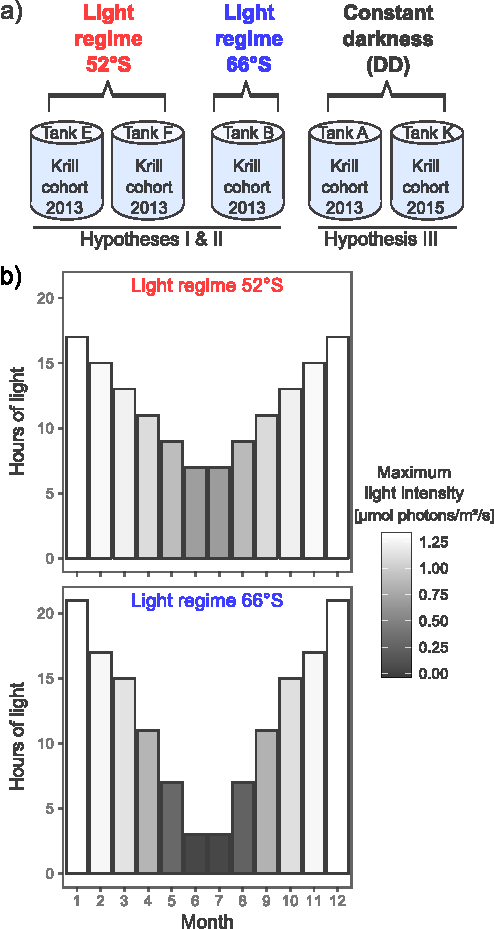
\includegraphics[height=10cm,keepaspectratio]{../Figures/Pub2_1.pdf}
        \caption{Long-term lab experiments at the Australian Antarctic Division: a) Experimental set-up and tested hypotheses, b) Simulated light regimes 55$^{\circ}$S and 66$^{\circ}$S.}
        \label{Pub2_1}
\end{figure}

However, due to increased mortality in tank A (treatment DD), an additional
tank for treatment DD (tank K) was set up in the beginning of March 2015 using
freshly caught Antarctic krill collected in 2015. The three different light
conditions were simulated within black lightproof plastic containers, one for
each experimental tank, using twin fluorescent tubes (Osram L18W/640 Cool
White) with a marine blue gel filter (Marine Blue 131; ARRI Australia Pty.
Ltd.). Light adjustment under treatments \SI{52}{\degree}S and
\SI{66}{\degree}S was carried out using a PC-controlled timer and dimming
system (\code{winDIM version 4.0e}; EEE, Portugal) with a maximum light
intensity of 100 lx (photon flux =
\SI{1.3}{\micro\mole\per\meter\square\per\second}) during midday in January
(corresponds to 1\% light penetration at \SI{30}{\meter} depth).  According to
the light regime, photoperiod and light-intensity profiles were adjusted at the
beginning of each month for each treatment. The simulated light-intensity
profiles for each treatment and month can be found in Supplementary Table S1.1 

The food level was held constant to remove that effect from our experiments
because we solely wanted to identify the effect that light regime had on the
seasonal cycle of Antarctic krill. Antarctic krill were fed daily between the
hours of 0830 and 0930 and the water flow in the tanks was turned off for
approximately 2 h to ensure feeding. The food comprised three live
laboratory-cultured algae (final concentrations were
\SI{1.5e4}{\cells\per\milli\liter} of \textit{Phaeodactylum tricornutum}
Bohlin, 1897, \SI{2e4}{\cells\per\milli\liter} of \textit{Geminigera cryophila}
(D.L. Taylor and C.C.  Lee) D.R.A. Hill, 1991,
\SI{2.2e4}{\cells\per\milli\liter} of \textit{Pyramimonas gelidicola} McFadden,
Moestrup and Wetherbee, 1982), three types of commercial algal paste
(\SI{1e4}{\cells\per\milli\liter} of \textit{Thalassiosira weissflogii}
(Grunow) G. Fryxell and Hasle, 1977 “TW 1200TM”,
\SI{5.1e4}{\cells\per\milli\liter} of Isochrysis Parke, 1949 “Iso 1800TM”,
\SI{4.8e4}{\cells\per\milli\liter} of Pavlova Butcher, 1952 “Pavlova 1800TM”;
Reed Mariculture, USA), and two types of prawn hatchery feeds (\SI{0.5}{\gram}
of FRiPPAK FRESH \#1CAR, \SI{0.5}{\gram} of FRiPPAK FRESH \#2CD; INVE,
Thailand).  Antarctic krill under treatment DD were fed in dim red light.
Moults and dead Antarctic krill were removed regularly from the tanks. 

Antarctic krill sampling of 6–10 individuals per tank and month was carried out
in the middle of each month during midday starting in February 2015 (for
treatment DD in dim red light). Due to different rates of mortality in the
tanks, the sampling scheme had to be adjusted during the course of the
experiment (Table \ref{Tab2_1}) to assure sampling over the whole experimental
period. Due to the problem with increased mortality under treatment DD
mentioned above, we decided to sample tanks A and K sequentially to ensure the
completion of the experiment over the 2-year period. 

% Please add the following required packages to your document preamble:
% \usepackage{booktabs}
\begin{table}[] \caption{Sampling scheme of the long-term experiment. Carapace
        length, digestive gland length and maturity score from these krill
        (\textit{E. superba}) were used for analysis of growth, feeding and
        maturity in this study. For lipid content analysis a reduced dataset
        was analysed.} 
        \label{Tab2_1}
{\scriptsize
\begin{tabular}{@{}llllllllll@{}}
\toprule
        \textbf{Treatment} & \textbf{Tank} & \textbf{Month 2-6} & \textbf{Month 7-13} & \textbf{Month 14-17} & \textbf{Month 18-19} & \textbf{Month 20-21} & \textbf{Month 22} & \textbf{Month 23} & \textbf{Month 24} \\ \midrule
52$^{\circ}$S      & E    & 10$\dagger$       & 6$\dagger$         & 6$\dagger$           & 6$\dagger$          &             & 8        &          &          \\
52$^{\circ}$S      & F    & 10        & 6          & 6            & 6           &             & 6        & 8        &          \\
66$^{\circ}$S      & B    & 10$\dagger$       & 6*$\dagger$        & 6$\dagger$           & 6$\dagger$          &             & 6        & 8        &          \\
DD        & A    & 10$\dagger$       & 6$\dagger$         & 6$\dagger$           &             &             &          &          &          \\
DD        & K    &           &            & 6            & 6$\dagger$          & 6           & 6        & 10       & 16       \\ \bottomrule
\end{tabular}
    \begin{tablenotes}
      \item Given numbers represent sampled individuals per month (n = 617).
      \item \textbf{*}: in July15 (month 7) one additional krill was sampled
      \item $\mathbf{\dagger}$: in April 15, July 15, October 15, January 16, April 16 and July 16 (months 4, 7, 10, 13, 16, 19) lipid content of 6 krill per month was analysed
     \end{tablenotes}

}
\end{table}


Live Antarctic krill was inspected under a stereomicroscope and the sex was
determined. Pictures of the carapace and the sexual organs (female thelycum and
male petasma) were taken with a Leica DFC 400 camera system (Leica
Microsystems, Germany). Carapace length (tip of the rostrum to posterior notch)
and digestive gland length (longest axis through carapace) were determined from
the pictures within the Leica \code{DFC Camera} software \code{version 7.7.1}
(Leica Microsystems, Switzerland). 

After visual inspection, the sampled Antarctic krill was immediately frozen in
liquid nitrogen. Frozen samples were stored at \SI{-80}{\celsius}.

The first inspection of the sex ratio within the experimental tanks revealed
that females dominated, with proportions of 71\%– 85\% per tank. 

\subsection{Growth analysis} 

Carapace length was used as a proxy for growth in the experiments. Antarctic
krill were sampled randomly from each experimental tank; thus, a general trend
observed in the carapace length data are assumed to display the general trend
of growth. 

The data analysis was performed in \code{RStudio version 1.0.136}
\citep{rstudio_team_rstudio:_2016}. Before the modelling process, a Pearson’s
product moment correlation was conducted to determine a potential difference in
growth pattern between male and female Antarctic krill; thus, the need for
separate models for each sex.  Due to the strong correlation (r = 0.82, p <
0.001) between males and females, based on the mean carapace length for each
sex across all treatments, data from both sexes were combined (n = 617). To
investigate the long-term trend (variable “time”) and the seasonal variability
(variable “month”) of Antarctic krill growth for each “treatment” (light
regime), a generalized additive mixed model (GAMM) with a Gaussian distribution
was used. An additive model was chosen over a linear one to resolve the
nonlinear relationship of the response and explanatory variables. The GAMM
takes the structure as specified by \citet{hastie_generalized_1987} and was
fitted using the gamm function in the mgcv package
\citep{wood_generalized_2006}. Random effects for “tank” were included in the
model to account for potential dependencies between individuals from the same
tank.  Prior to the modelling process, temporal autocorrelation was examined
using the acf function in \code{R}. Time series are often subject to
latitudinal dependencies between data points and not accounting for the
autocorrelation can result in biased estimates of model parameters
\citep{panigada_modelling_2008}. As autocorrelation was neither detected, nor
evident in residual analysis during model validation, no temporal
autocorrelation term was included in the final model. 

Smoothed terms were fitted as regression splines (variable “time”), apart for
the variable “month”, which was modelled using cyclic cubic regression splines,
setting knots manually between 1 (January) and 12 (December) to account for the
circular nature of this term. Differences in temporal pattern between the three
light regimes (\SI{52}{\degree}S, \SI{66}{\degree}S, DD) were implemented using
the by- argument of the gamm function, which allows for the creation of
separate smoothers for each level of the treatment factor (light regime) over
the temporal variables “month” and “time”. Hence, separate parameter estimates
for the temporal variables are obtained for each treatment level. To avoid
overfitting, the smooth function of the variable “month” was manually
restricted to k = 5. Model selection was conducted using manual
stepwise-backward selection based on Akaike’s information criterion (AIC)
\citep{akaike_likelihood_1981}. If the addition of a term led to an AIC
decrease of >2 per degree of freedom, or an increase of the adjusted R2, or if
the term was significant, then the term was included in the model. Model fit
was examined by residual analysis.

\subsection{Feeding Analysis}

The feeding index (\%) was calculated as digestive gland length $\times$
(carapace length)-1 $\times$ 100. Data of males and females were combined
because of the strong correlation of monthly mean values (Pearson’s product
moment correlation, r = 0.95, p < 0.001). To investigate a temporal pattern in
the feeding index of Antarctic krill for each treatment, a GAMM was employed as
described above (section Growth analysis). The smooth function of the variable
“time” was manually restricted to k = 6.

\subsection{Lipid content analysis}

Every 3 months from April 2015 to July 2016, six replicate samples from each
treatment were tested for their lipid content. Lipids were extracted from the
carapace, which was separated from the frozen samples with a scalpel on dry ice
prior to extraction. Lipid extraction was performed with
dichloromethane:methanol (2:1, v:v) according to the method described by
\citet{hagen_lipids_2000}. Lipid content was determined gravimetrically and was
calculated in percentage of dry mass. One data point (sample code “Jan16\_E04”)
was removed due to the negative value of lipid content that indicated incorrect
measurement for that individual. 

Lipid content differed between male and female Antarctic krill (Pearson’s
product moment correlation of pooled monthly mean values, r = 0.26, p = 0.62);
therefore, statistical analysis was performed separately for each sex. Data for
males were not sufficient for robust modelling and only females were considered
for this analysis (n = 83). Only one tank for each time point and treatment was
available, therefore a mixed model to resolve a potential tank effect could not
be employed. For treatment DD, five samples were available from a second tank,
but these were not sufficient for the inclusion of a random effect. Therefore,
a generalized additive model (GAM) was employed to examine the temporal pattern
of female Antarctic krill lipid content, following the protocol described in
section Growth analysis. The smooth function of the variable “time” was
manually restricted to k = 6. Because the variable “month” was not significant,
it was excluded from the final model.

\subsection{Maturity Analysis}

The maturity stage of the sampled Antarctic krill was assessed by analysing
pictures of the external sexual organs according to \citet{makarov_stages_1980}
and \citet{thomas_thelycum_1987}. A maturity score was assigned using the
method of \citet{brown_temperature_2010, brown_flexible_2011}. Due to the
ordinal characteristic of the maturity scores, Pearson correlation of monthly
mean values could not be per- formed with the data set. Therefore, we visually
inspected the relationship between maturity score and hours of light in males
and females. Seasonal maturity scores differed between male and female
Antarctic krill (Fig. \ref{Pub2_2}); therefore, statistical analysis was
performed on females only (n = 493), as there were not sufficient data to allow
for modelling males separately. To investigate the temporal pattern of maturity
of female Antarctic krill for each treatment, a GAMM was employed as described
in section Growth analysis. Because model residuals were autocorrelated, an
auto-regressive correlation structure of the order 1 was added, which improved
model fit and resolved the dependencies between residuals. Maturity scores are
represented as whole numbers and take values between 3 and 5. Therefore, the
GAMM was initially modelled using a Poisson distribution with a logarithmic
link function between predictor and response. Due to overdispersion, a negative
binomial GAMM had to be used. The smooth function of the variable “time” was
manually restricted to k = 6. 

%%%%%%%% Figure 2
\begin{wrapfigure}{O}{0.4\textwidth}
       \vspace{-20pt}
        \centering
        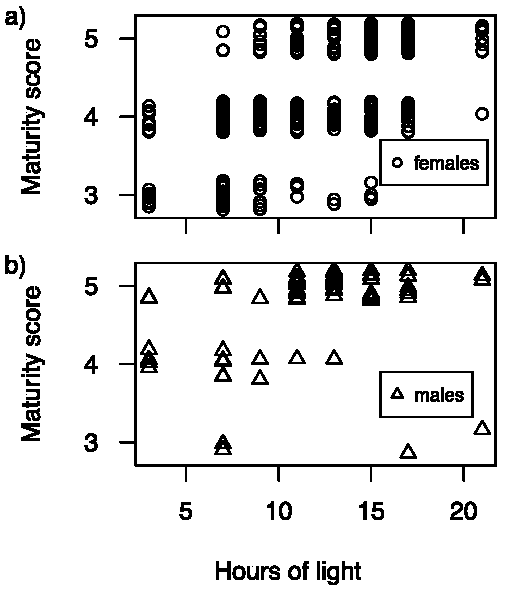
\includegraphics[width=0.35\textwidth]{../Figures/Pub2_2.pdf}
        \vspace{-15pt}
        \caption{Relationship between maturity score and hours of light in a)
        females and b) males.}
        \label{Pub2_2}
         \vspace{-10pt}
\end{wrapfigure}

To examine differences in the critical photoperiod between latitudinal light
regimes 52$^{\circ}$S and 66$^{\circ}$S, a logistic regression was used. As
only full maturity was investigated, maturity scores <5 were set to zero and
full maturity (score = 5) was set to one in all samples, resulting in a data
set of zeros and ones. The relationship between full maturity of female
Antarctic krill and photoperiod was modelled with a binomial generalized linear
mixed model (GLMM) with a logit function between predictor and response and an
interaction term for factor “treatment” and continuous variable “hours of
light”. The model was fitted using the glmer function from the lme4 library. To
account for dependencies between individuals from the same tank, random effects
for “tank” were included in the model. Model fit was assessed by constructing a
receiver operating characteristic (ROC) curve using the pROC package in R,
where the area under the curve (AUC) indicates the goodness of fit
\citep{boyce_evaluating_2002}. Values below 0.7 are considered poor and 1.0
represents a perfect fit \citep{cumming_using_2000}. The critical photoperiod
(= photoperiod, when the probability to be fully mature is 50\%) was predicted
from the 95\% confidence intervals.

\subsection{Data archiving} 

Processed data have been uploaded to the database PANGAEA and can be accessed
under \url{https://doi.pangaea.de/10.1594/PANGAEA.885889.}

\section{Results}

\subsection{Growth Analysis} 

Carapace length ranged from 8.1 to 19.02 mm with a mean ($\pm$SD) of 11.71 mm
($\pm$1.61 mm) across the whole data set. The GAMM (model M1; Table
\ref{Tab2_2}) revealed significant seasonal and interannual patterns in growth,
which were similar across all treatments (Figs. \ref{Pub2_3}a, \ref{Pub2_3}b).
Shrinkage was observed in the beginning of the experiments. A significant
seasonal variability with shrinkage towards austral winter (June to August) and
growth towards austral summer (December to February) was observed under
treatments 52$^{\circ}$S and DD (not significant under treatment
66$^{\circ}$S).

%%%%%%%% Figure 3
\begin{figure}[ht!]
        \centering
        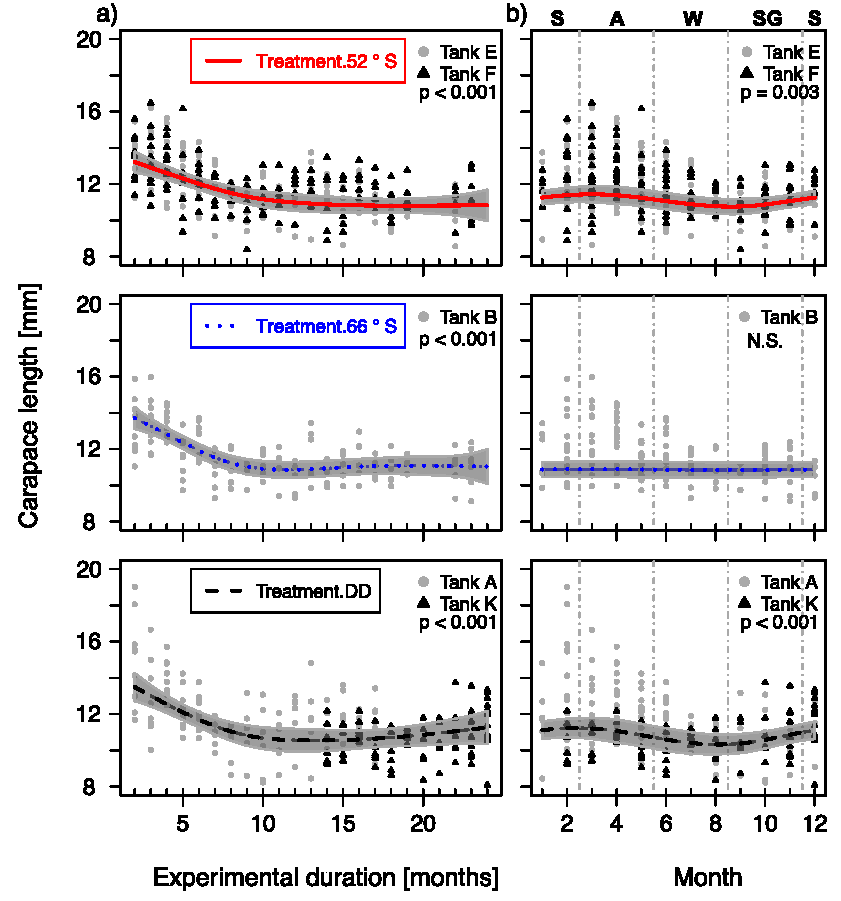
\includegraphics[width=0.85\textwidth]{../Figures/Pub2_3.pdf}
        \caption{Estimated smooth terms of the GAMM for carapace length within
        treatments 52$^{\circ}$S, 66$^{\circ}$S and DD with a) explanatory
        variable time (thin plate regression spline smooth term) showing the
        general trend over the whole experimental period and b) explanatory
        variable month (cyclic smooth term) representing the seasonal trend
        over the months of the year. The smoothers (lines) are displayed with
        95\% confidence intervals (shading), the raw data points for
        experimental tanks (shapes) and the p-value. The seasonal periods are
        indicated by vertical dashed lines and the following abbreviations: SG
        - spring, S - summer, A - autumn, W - winter.}
        \label{Pub2_3}
\end{figure}

\begin{table}[]
\centering
{\scriptsize
\caption{Model results, showing model statistics for parametric coefficients (estimates, standard errors (SD), \textit{z}- or \textit{t}-values and \textit{p}-values), a measure of explained variance of the model (Deviance or Adjusted $R^{2}$ (Adj. $R^{2}$)) and non-parametric terms where applicable (estimated degrees of freedom (edf), \textit{F}-statistic and \textit{p}-values). }
\label{Tab2_2}
\begin{tabular}{@{}lllllll@{}}
\toprule \\
\textbf{Intercept} & \textbf{Estimate} & \textbf{SD} & \textbf{\textit{t}-value} & \textbf{\textit{p}-value} & \textbf{Adj. R}$\mathbf{^{2}}$ & \\
\textbf{M1} & $11.67$ & $0.12$ & $101$ & $<0.001$ & $0.39$ & \\
\midrule
& \multicolumn{2}{c}{Treatment 52$^{\circ}$S} & \multicolumn{2}{c}{Treatment 66$^{\circ}$S} & \multicolumn{2}{c}{Treatment DD} \\
% M1 Test
\textbf{Variable} & \cellcolor{gray!50}\textbf{Time} & \cellcolor{gray!50}\textbf{Month} &\cellcolor{blue!25}\textbf{Time} & \cellcolor{blue!25}\textbf{Month} & \cellcolor{blue!50}\textbf{Time} & \cellcolor{blue!50}\textbf{Month} \\

\textbf{Smooth (edf)} & \cellcolor{gray!50}2.84 & \cellcolor{gray!50}1.74 &\cellcolor{blue!25}3.56 & \cellcolor{blue!25}0.39 & \cellcolor{blue!50}3.32 & \cellcolor{blue!50}1.8 \\

\textbf{F-value} & \cellcolor{gray!50}32.8 & \cellcolor{gray!50}1.95 &\cellcolor{blue!25}20.65 & \cellcolor{blue!25}0.15 & \cellcolor{blue!50}20.31 & \cellcolor{blue!50}2.46 \\

\textbf{p-value} & \cellcolor{gray!50}<0.001 & \cellcolor{gray!50}0.003 &\cellcolor{blue!25}<0.001 & \cellcolor{blue!25}0.13 & \cellcolor{blue!50}<0.001 & \cellcolor{blue!50}<0.001 \\

\midrule
% M2 Test
\textbf{Intercept} & \textbf{Estimate} & \textbf{SD} & \textbf{\textit{t}-value} & \textbf{\textit{p}-value} & \textbf{Adj. R}$\mathbf{^{2}}$ & \\
\textbf{M2} & $42.08$ & $0.22$ & $189.8$ & $<0.001$ & $0.64$ & \\
\midrule

\textbf{Variable} & \cellcolor{gray!50}\textbf{Time} & \cellcolor{gray!50}\textbf{Month} &\cellcolor{blue!25}\textbf{Time} & \cellcolor{blue!25}\textbf{Month} & \cellcolor{blue!50}\textbf{Time} & \cellcolor{blue!50}\textbf{Month} \\

\textbf{Smooth (edf)} & \cellcolor{gray!50}2.87 & \cellcolor{gray!50}5.09 &\cellcolor{blue!25}2.55 & \cellcolor{blue!25}1.47 & \cellcolor{blue!50}3.13 & \cellcolor{blue!50}2.79 \\

\textbf{F-value} & \cellcolor{gray!50}41.42 & \cellcolor{gray!50}4.2 &\cellcolor{blue!25}92.84 & \cellcolor{blue!25}0.39 & \cellcolor{blue!50}64.52 & \cellcolor{blue!50}1.4 \\

\textbf{p-value} & \cellcolor{gray!50}<0.001 & \cellcolor{gray!50}<0.001 &\cellcolor{blue!25}<0.001 & \cellcolor{blue!25}0.041 & \cellcolor{blue!50}<0.001 & \cellcolor{blue!50}<0.001 \\
\midrule
% M3 Test
\textbf{Intercept} & \textbf{Estimate} & \textbf{SD} & \textbf{\textit{t}-value} & \textbf{\textit{p}-value} & \textbf{Deviance} & \\
\textbf{M3} & $17.21$ & $0.77$ & $22.33$ & $<0.001$ & $50.9\%$ & \\
\midrule

\textbf{Variable} & \cellcolor{gray!50}\textbf{Time} & \cellcolor{gray!50} &\cellcolor{blue!25}\textbf{Time} & \cellcolor{blue!25} & \cellcolor{blue!50}\textbf{Time} & \cellcolor{blue!50} \\

\textbf{Smooth (edf)} & \cellcolor{gray!50}3.58 & \cellcolor{gray!50} &\cellcolor{blue!25}3.82 & \cellcolor{blue!25} & \cellcolor{blue!50}1.0 & \cellcolor{blue!50} \\

\textbf{F-value} & \cellcolor{gray!50}1.16 & \cellcolor{gray!50} &\cellcolor{blue!25}14.97 & \cellcolor{blue!25} & \cellcolor{blue!50}0.05 & \cellcolor{blue!50} \\

\textbf{p-value} & \cellcolor{gray!50}0.3 & \cellcolor{gray!50} &\cellcolor{blue!25}<0.001 & \cellcolor{blue!25} & \cellcolor{blue!50}0.82 & \cellcolor{blue!50} \\
\midrule

% M4 Test
\textbf{Intercept} & \textbf{Estimate} & \textbf{SD} & \textbf{\textit{t}-value} & \textbf{\textit{p}-value} &  \textbf{Adj. R}$\mathbf{^{2}}$ & \\
\textbf{M4} & $1.43$ & $0.01$ & $134.9$ & $<0.001$ & $0.45$ & \\
\midrule

\textbf{Variable} & \cellcolor{gray!50}\textbf{Time} & \cellcolor{gray!50}\textbf{Month} &\cellcolor{blue!25}\textbf{Time} & \cellcolor{blue!25}\textbf{Month} & \cellcolor{blue!50}\textbf{Time} & \cellcolor{blue!50}\textbf{Month} \\

\textbf{Smooth (edf)} & \cellcolor{gray!50}1.0 & \cellcolor{gray!50}4.14 &\cellcolor{blue!25}1.88 & \cellcolor{blue!25}4.07 & \cellcolor{blue!50}3.33 & \cellcolor{blue!50}2.88 \\

\textbf{F-value} & \cellcolor{gray!50}6.1 & \cellcolor{gray!50}15.0 &\cellcolor{blue!25}5.84 & \cellcolor{blue!25}7.7 & \cellcolor{blue!50}4.58 & \cellcolor{blue!50}1.19 \\

\textbf{p-value} & \cellcolor{gray!50}0.014 & \cellcolor{gray!50}<0.001 &\cellcolor{blue!25}0.002 & \cellcolor{blue!25}<0.001 & \cellcolor{blue!50}0.04 & \cellcolor{blue!50}<0.001 \\
\midrule
\textbf{M5} & \textbf{Estimate} & \textbf{SD} & \textbf{\textit{z}-value} & \textbf{\textit{p}-value} &  \textbf{AUC} & \\
\textbf{Intercept} & $-6.09$ & $0.78$ & $-7.86$ & $<0.001$ & $0.77$ & \\
\textbf{Hours of Light} & $0.49$ & $0.06$ & $7.86$ & $<0.001$ & & \\
\textbf{Treatment} & $1.22$ & $1.25$ & $0.98$ & $0.4$ & & \\
\textbf{Interaction: Light * Latitude} & $-0.16$ & $0.09$ & $-1.73$ & $0.084$ & & \\

\bottomrule
\end{tabular}
    \begin{tablenotes}
      \item Significant \textit{p}-values of explanatory variables are in bold.
      \item \textbf{M1}: GAMM for carapace length over time for each treatment with random effects for tank
      \item \textbf{M2}: GAMM for feeding index over time for each treatment and random effects for tank
      \item \textbf{M3}: GAM for lipid content of females over time for each treatment 
      \item \textbf{M4}: Negative binomial GAMM for female maturity over time for each treatment with random effects for tank and AR1-correlation structure
      \item \textbf{M5}: Binomial GLMM for full maturity of females in relation to hours of light with interaction term for treatment (52$^{\circ}$S and 66$^{\circ}$S) and random effects for tank effect, AUC = ‘Area under the curve’ from ROC-curve analysis serves as an indication of model fit
    \end{tablenotes}
}
\end{table}


\subsection{Feeding}

The feeding index data ranged from 25.15\% to 66.09\% with a mean ($\pm$SD) of
42.00\% ($\pm$6.58\%). 

The GAMM revealed significant changes in the feeding index over time (model M2;
Table 2). We observed an increase of the feeding index throughout the
experimental period in all treat- ments and a final stagnation in treatments
52$^{\circ}$S and DD (Figs. \ref{Pub2_4}a, \ref{Pub2_4}b). The seasonal trend
differed between treatments. In treatment 52$^{\circ}$S, the feeding index
strongly increased during the autumn period (March to May) with a subsequent
decrease and stabilization during the rest of the year. The seasonal trend in
treatment 66$^{\circ}$S was very weak and will therefore not be described
further. In treatment DD, the feeding index increased over a longer period
(March to July) and decreased during the rest of the year.

%%%%%%%%%% Figure 4
\begin{figure}[htb!]
        \centering
        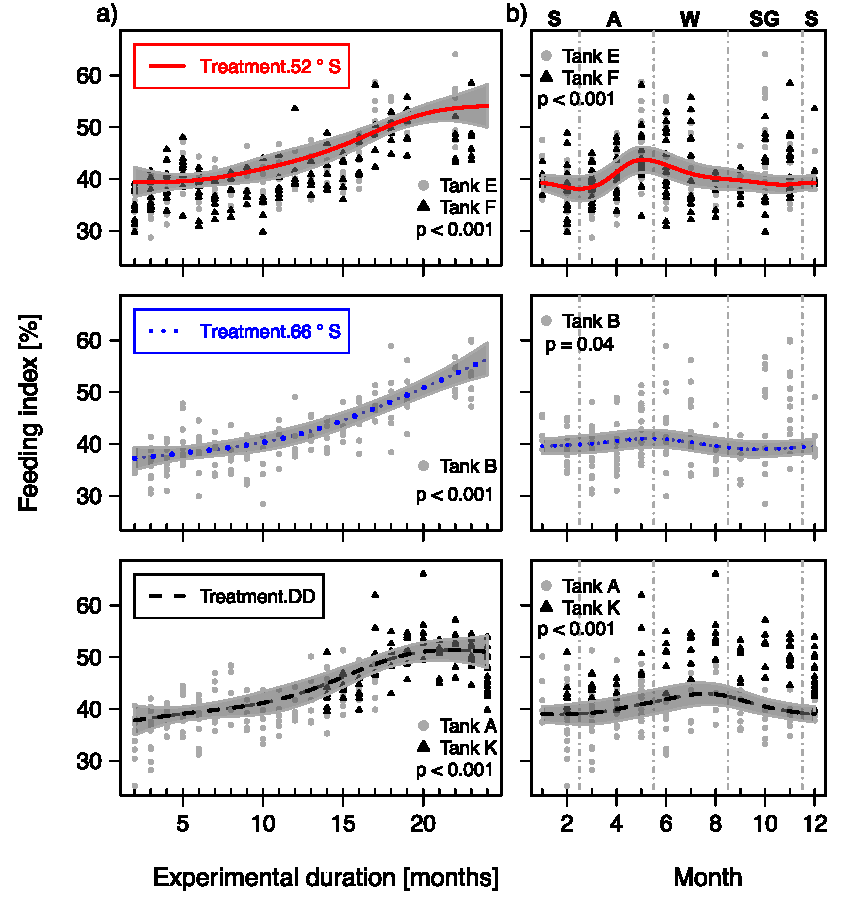
\includegraphics[width=0.85\textwidth]{../Figures/Pub2_4.pdf}
        \caption{Estimated smooth terms of the GAMM for feeding index within
        treatments 52$^{\circ}$S, 66$^{\circ}$S and DD with a) explanatory
        variable time (thin plate regression spline smooth term) showing the
        general trend over the whole experimental period and b) explanatory
        variable month (cyclic smooth term) representing the seasonal trend
        over the months of the year. The smoothers (lines) are displayed with
        95\% confidence intervals (shading), the raw data points for
        experimental tanks (shapes) and the p-value. The seasonal periods are
        indicated by vertical dashed lines and the following abbreviations: SG
        - spring, S - summer, A - autumn, W - winter.}
        \label{Pub2_4}
\end{figure}

%%%%%%%%%%% Figure 5
\begin{figure}
        \centering
        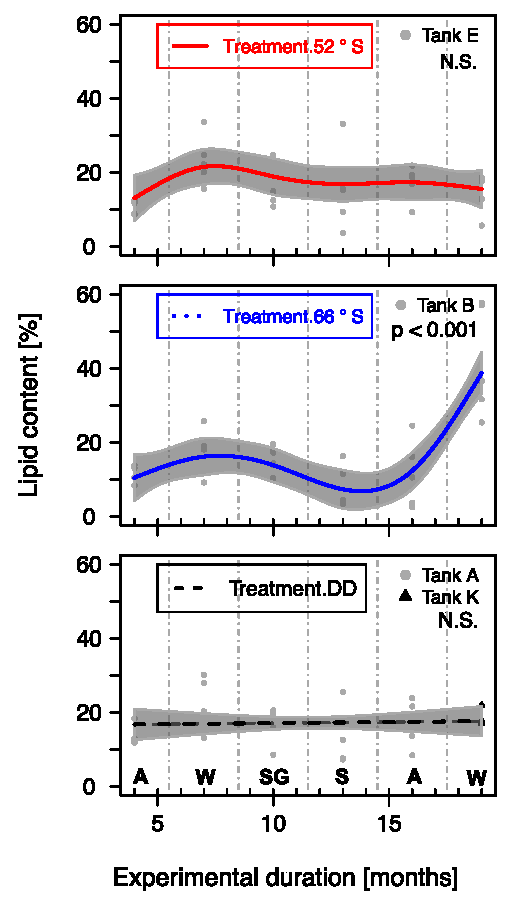
\includegraphics[width=0.75\textwidth]{../Figures/Pub2_5.pdf}
        \caption{Estimated smooth terms of the GAM for lipid content in females
        within treatments 52$^{\circ}$S, 66$^{\circ}$S and DD. The explanatory
        variable time (thin plate regression spline smooth term) is showing the
        general trend over the whole experimental period. The smoothers (lines)
        are displayed with 95\% confidence intervals (shading), the raw data
        points for experimental tanks (shapes) and the p-value. The seasonal
        periods are indicated by vertical dashed lines and the following
        abbreviations: SG - spring, S - summer, A - autumn, W - winter.}
        \label{Pub2_5}
\end{figure}

\subsection{Lipids}

The lipid content data of males and females ranged from 2.53\% to 57.75\% with
a mean ($\pm$SD) of 17.04\% ($\pm$9.12\%). The GAM considering female lipid
content data only (model M3; Table 2) revealed significant differences in
temporal variability of lipid content be- tween the experimental treatments
(Fig. \ref{Pub2_5}). Even though the variable “month” was not significant, a
resembling seasonal pattern was observed in the interannual trend under
treatment 66$^{\circ}$S with an increase towards austral winter and a decrease
towards austral summer. The increase of lipid content during the second winter
was much stronger than the first winter. No significant patterns were found for
treatments 52$^{\circ}$S and DD.

\subsection{Maturity}

Implementing the negative binomial GAMM for female maturity (model M4; Table
2), we found a significant seasonal cycle of maturity under treatments
52$^{\circ}$S, 66$^{\circ}$S, and DD with sexual regression towards austral
winter and sexual re-maturation towards austral spring and summer (Figs.
\ref{Pub2_6}a, \ref{Pub2_6}b). Significant interannual patterns differed
between treatments. In treatments 52$^{\circ}$S and 66$^{\circ}$S, a slight
decrease of maturity over the whole study period was observed. The interannual
pattern in treatment DD showed that sexual regression was only completed during
the first winter of the experiments. 


%%%%%%%%%%% Figure 6
\begin{figure}
        \centering
        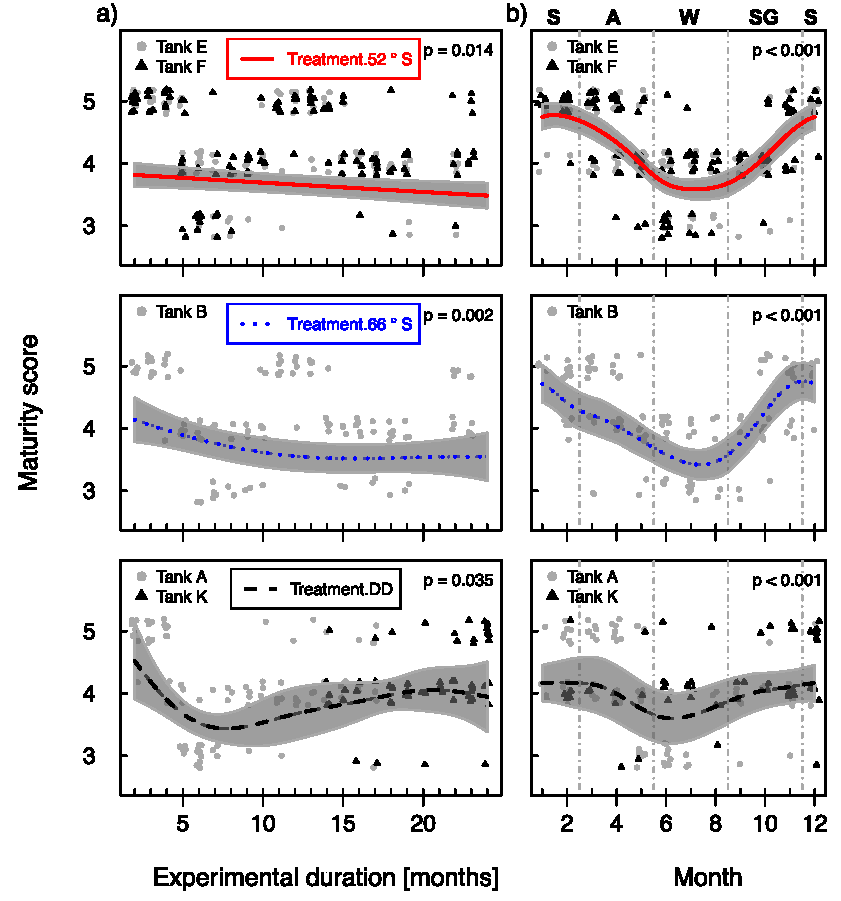
\includegraphics[width=0.85\textwidth]{../Figures/Pub2_6.pdf}
        \caption{Estimated smooth terms of negative binomial GAMM for female
        maturity within treatments 52$^{\circ}$, 66$^{\circ}$S and DD with a)
        explanatory variable time (thin plate regression spline smooth term)
        showing the general trend over the whole experimental period and b)
        explanatory variable month (cyclic smooth term) representing the
        seasonal trend over the months of the year. The smoothers (lines) are
        displayed with 95\% confidence intervals (shading), the jittered raw
        data points for experimental tanks (shapes) and the p-value. The
        seasonal periods are indicated by vertical dashed lines and the
        following abbreviations: SG - spring, S - summer, A - autumn, W -
        winter.}
        \label{Pub2_6}
\end{figure}

The binomial GLMM (model M5; Table 2) suggests that the variable “hours of
light” significantly affects female maturity in treatments 52$^{\circ}$S and
66$^{\circ}$S. The interaction term between “hours of light” and “treatment”
was marginally not significant. When investigating the critical photoperiod at
the probability of 50\%, differences between the treatments were found (Fig.
\ref{Pub2_7}). For treatment 52$^{\circ}$S, the critical photoperiod was
estimated as 12.5 h of light with 95\% confidence intervals (11.86, 13.22). For
treatment 66$^{\circ}$S, an estimate of 14.76 h of light with 95\% confidence
intervals (13.3, 16.3) was found.


%%%%%%%%%%% Figure 7

\begin{wrapfigure}{O}{6cm}
        \centering
        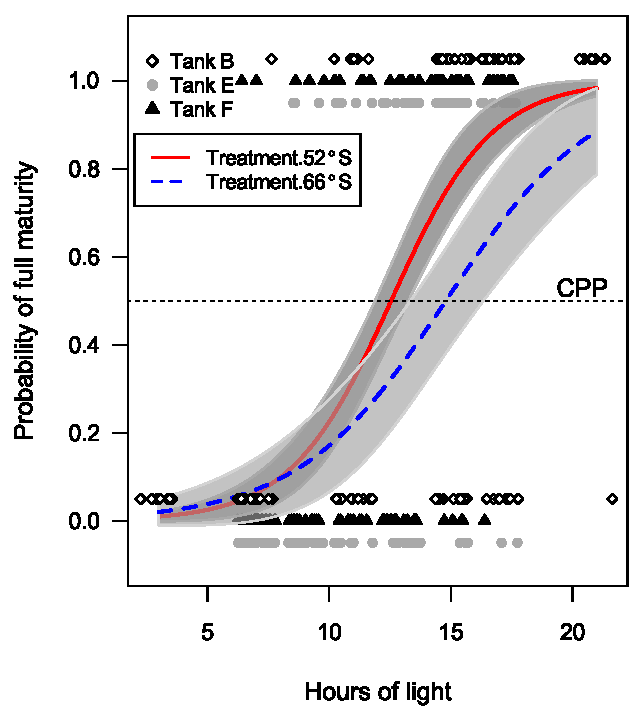
\includegraphics[height=7cm, keepaspectratio]{../Figures/Pub2_7.pdf}
        \caption{Results from the logistic regressions for 52$^{\circ}$S and
        66$^{\circ}$S: Estimated trends of the binomial GLMM (lines) are shown
        with 95\% confidence intervals (shading) and jittered raw data points
        for experimental tanks (shapes). The horizontal line indicates the 50\%
        probability level for the critical photoperiod (CPP).}
        \label{Pub2_7}
\end{wrapfigure}

\section{Discussion}

We present findings from the first 2-year laboratory experiments investigating
the effect of light regime and the biological clock on the seasonal cycle of
Antarctic krill. 

The observed seasonal cycles of growth, feeding, lipid metabolism, and maturity
under the simulated latitudinal light regimes suggest that light regime is an
essential zeitgeber for Antarctic krill. The occurrence of a pronounced lipid
cycle under treatment 66$^{\circ}$S and the observed differences in critical
photoperiods for the maturation cycle indicate that Antarctic krill may respond
flexibly to different latitudinal light regimes. This may represent an adaptive
mechanism to the extreme light regimes in the Southern Ocean and ensure
survival of Antarctic krill in different latitudinal habitats, especially
during winter. Moreover, seasonal patterns of growth, feeding, and maturity
persisted under constant darkness indicating the presence of an endogenous
timing system modulating these rhythms. High food supply does not suppress
endogenously driven seasonal rhythms of growth, feeding, lipid metabolism, and
maturity. 

The following considerations should be taken into account when interpreting the
findings of this study. Due to limits in space and costs for the long-term
laboratory experiments and variable mortality rates in the tanks, we had to
adjust the experimental set-up and sampling scheme accordingly. This led to a
sampling design with replication in experimental units over the full study
period for treatment 52$^{\circ}$S only. Carapace length, digestive gland
length, and maturity data from treatment 66$^{\circ}$S and partly treatment DD,
as well as the lipid content data set, may be regarded as pseudoreplicated
\citep{colegrave_using_2018} because the replication in experimental units over
the full study period is incomplete. We have included the random effect
“experimental tank” in our models, where appropriate, during statistical
analysis of the data to account for a potential tank effect as far as possible.
How- ever, we cannot exclude that differences in tank and replicate number may
have influenced the results of our tests. 

To interpret the response of Antarctic krill to constant darkness over the full
2-year period, we combined data from two different cohorts of Antarctic krill.
The “new” cohort was acclimated to the laboratory conditions for 1 year, before
sampling started. Preliminary analysis revealed similar trends in both cohorts
under constant darkness, which supports our assumption that both cohorts
responded similarly to the treatment. 

Moreover, we decided to solely analyse a reduced data set for lipid content
because frozen Antarctic krill samples from the 2-year experiments are very
valuable and can be used for multiple analyses. The reduced data set is
adequate to display the pronounced seasonal lipid cycle under the high
latitudinal light regime, but it may be insufficient to test for weaker
patterns in the other treatments. Since potential differences in the male
pattern were indicated and the number of males was too low to conduct a
separate analysis, we decided to analyse females only for lipid content and
maturity. 

Moreover, we presume that the observations made in the first few months of the
experiment represent a general period of acclimation to the experimental
conditions. It may explain the strong shrinkage, suppressed lipid accumulation,
and a general similarity of the data under all treatments in the beginning of
the experiments. 

Our observation of a seasonal cycle of growth confirms findings by
\citet{brown_temperature_2010} that suggest growth is influenced by light
regime, independently of food supply. For the first time, we show that
Antarctic krill’s growth cycle is endogenous and persists under constant
darkness. The observed shrinkage in autumn and winter in this study may be
partly related to the maturity cycle.  Females have been observed to shrink
during sexual regression \citep{thomas_thelycum_1987} and
\citet{tarling_growth_2016} suggested that it might be explained by
morphometric changes due to the contraction of the ovaries. On the other hand,
the shrinkage may reflect an overwintering mechanism
\citep{quetin_behavioral_1991}.  This is sup- ported by our observation of
significant seasonal shrinkage under constant darkness where we did not find a
pronounced maturity cycle over the 2-year period. 

The seasonal increase of feeding in autumn, which was observed under treatment
52$^{\circ}$S, may represent an inherent strategy to be able to accumulate
enough lipid stores for winter \citep{hagen_lipid_2001, meyer_seasonal_2010}.
These results partly agree with the short-term study by
\citet{teschke_simulated_2007} who observed higher clearance rates under autumn
and summer light conditions compared with constant darkness, suggesting
enhanced feeding activity under light conditions of prolonged day length. The
comparability of both studies may be limited because we solely used a
morphometric index as a measure of feeding activity. The feeding index may be
biased by the strong shrinkage that occurred in the beginning of our
experiments, which could have masked a suppressed feeding activity in the first
months. In our long-term study, the seasonal feeding trend under treatment DD
resembled the other treatments with a shift of peak feeding activity towards
winter that may indicate an endogenous control of seasonal feeding activity in
Antarctic krill. The general increase of feeding index during the experiments
suggests that Antarctic krill is able to make use of food supply throughout the
whole experimental period. This observation may also indicate a flexible
feeding behaviour of Antarctic krill \citep{atkinson_feeding_2002} that has
also been observed in the field in winter \citep{quetin_behavioral_1991,
huntley_elemental_1994, schmidt_feeding_2014}.

In our study, we observed a seasonal pattern of lipid content under treatment
66$^{\circ}$S that may be stimulated by the high latitudinal light regime. It
resembles the lipid cycle observed in the field with highest values of lipid
content in autumn and lowest values in early spring \citep{hagen_lipid_2001,
meyer_seasonal_2010}. This is the first study that shows the possible influence
of light regime on the lipid cycle in Antarctic krill. The accumulation of
lipid reserves may be adjusted according to the latitudinal light regime, which
may explain the differences observed in the field with higher lipid stores
found in regions at higher latitudes \citep{schmidt_feeding_2014}. We also
observed a match of the period of lipid depletion and re-maturation, which
supports the assumption that lipid stores may be used for the maturation
process \citep{teschke_effects_2008}.

The effect of light regime on the maturity cycle \citep{hirano_antarctic_2003,
teschke_effects_2008, brown_flexible_2011} is confirmed by our study. The
endogenous cycle of maturity under constant darkness has been observed in
short-term experiments before \citep{thomas_thelycum_1987,
kawaguchi_learning_2007, brown_flexible_2011}. We show that this pattern does
not persist during the second year under constant darkness and suggest that the
zeitgeber photoperiod is required for the entrainment of the maturity cycle
over longer periods. Results from former experiments
\citep{hirano_antarctic_2003, brown_flexible_2011} indicate that Antarctic
krill’s maturity cycle may be entrained by the timing of two contrasting
photoperiods (peak and trough light regimes). 

To study potential differences in the physiological response of Antarctic krill
to different latitudinal light regimes, we used the critical photoperiod
(defines the day length when 50\% of the population shift from one state to
another, here maturity) as an indicator to determine the time of the year that
is a turning point in the seasonal cycle. However, using critical photoperiod,
we cannot give rise to any conclusion regarding the mechanism of entrainment of
these rhythms. We observed that the critical photo- period for maturity
differed between latitudinal light regimes, being higher under the high
latitudinal light regime. An increase of critical photoperiod with latitude has
also been found in insects in relation to diapause
\citep{bradshaw_evolution_2007, tyukmaeva_adaptation_2011,
hut_latitudinal_2013}. Organisms with higher critical photo- periods have an
adaptive advantage under the extreme seasonal changes of photoperiod at higher
latitudes where they have to prepare early enough to ensure survival during
winter. Specifically, a higher critical photoperiod for maturity implies that
Antarctic krill is able to undertake the critical stage of sexual regression
and re-maturation during the time of the year when photoperiods are longer
compared with regions at lower latitudes. In regions with extreme changes of
photoperiod and severe winter conditions, this adaptive mechanism may ensure
that Antarctic krill prepares early enough for winter and keeps up
energy-saving mechanisms long enough. 

Antarctic krill’s flexibility in adjusting its photoperiodic response to a wide
range of latitudinal light regimes may be advantageous under future climate
change, as a southward migration trend of Antarctic krill to higher latitudes
at the western Antarctic Peninsula has been reported \citep{ross_trends_2014}.
Still, changes in sea-ice dynamics, such as the timing of sea-ice formation or
melt, may lead to mismatches in the timing of critical life-cycle events
\citep{clarke_climate_2007}. For instance, an earlier phytoplankton bloom
associated with earlier sea-ice melt may influence the survival and
reproductive success of Antarctic krill. Therefore, its potential to adapt to
future environmental changes may also depend on its genetic flexibility in
adjusting its photoperiodic response and the timing of critical life-cycle
events \citep{bradshaw_evolution_2007}.

Our findings support the assumption of a circannual timing system synchronized
by light regime in Antarctic krill (Meyer 2011). The modulation of seasonal
rhythms of growth, feeding, lipid metabolism, and maturity happen independently
of constant food supply, indicating an inherent mechanism in Antarctic krill
that regulates the timing of these processes according to the light regime.
Photoperiod may play a significant role in the initiation of neuroendocrine
cascades (on–off mechanism) in Antarctic krill, as it has been found to be the
primary signal initiating diapause, migration, or reproduction in other
arthropods \citep{bradshaw_evolution_2007}. It remains to be clarified if the
photoperiodic time measurement inducing seasonal events in Antarctic krill is
related to the circadian clock \citep{hut_latitudinal_2013,
meuti_functional_2015} or represents an independent circannual timing system.
Using light regime as a seasonal zeitgeber makes ecologically sense because it
is a more reliable cue than food availability. The intensity of the initiated
seasonal physiological processes may be regulated in the field by the
interaction with other factors such as food or temperature. High food quality
and quantity were found to advance growth \citep{ross_growth_2000,
atkinson_natural_2006} and maturation \citep{quetin_environmental_2001} in
Antarctic krill. We propose that this effect is restricted to specific seasonal
periods that are determined by the response of Antarctic krill’s endogenous
timing system to the exposed latitudinal light regime. 

This study has high relevance for future modelling approaches of Antarctic
krill densities in the Southern Ocean, especially under the aspect of climate
change. Recent Antarctic krill models have focussed on intraspecific food
competition \citep{ryabov_competition-induced_2017} or have been conducted on a
conceptual basis \citep{groeneveld_how_2015}. The incorporation of light regime
into dynamic models may significantly improve the predictability of growth,
energy budget, and reproduction in Antarctic krill. Recently, a coupled
energetics and moult-cycle model has been developed for Antarctic krill that
considered resource allocation based on the seasonal cycles of growth and
maturity \citep{constable_modelling_nodate}. Further research on the phenology
and biological clock of Antarctic krill will help to better understand its
adaptive potential to environmental changes. 

\section{Conclusion}

This study aimed to investigate the impact of light regime on Antarctic krill’s
phenology and the role of its endogenous timing system. Our observations
suggest that light regime affects seasonal cycles of growth, feeding, lipid
metabolism, and maturity under constantly high food supply. Antarctic krill
possesses an endogenous timing system that maintains seasonal rhythms un- der
constant darkness and is most likely entrained by light regime. Varying
critical photoperiods under different latitudinal light regimes indicate that
this timing system is flexible, allowing Antarctic krill to adjust its
physiological and behavioural responses to the extreme light conditions in the
Southern Ocean. 

\section{Acknowledgements}

We thank the staff at the Australian Antarctic Division (namely R. King, T.
Waller, A. Cooper, and B. Smith) for their advice and the maintenance of the
Antarctic krill during the long-term experiments in the Antarctic krill
aquarium. Sincere thanks go to F. Piccolin and F. Müller for their help in
setting up the experiment and their collegial support. M. Vortkamp is
acknowledged for her help in the laboratory during lipid content analysis. This
study was funded by the Helmholtz Virtual Institute “PolarTime” (VH-VI-500:
Biological timing in a changing marine environment — clocks and rhythms in
polar pelagic organisms), the ministry of science and culture (MWK) of Lower
Saxony, Germany (Research Training Group “Interdisciplinary approach to
functional bio- diversity research” (IBR)), and Australian Antarctic Program
Project \#4037. Additional funds were made available via the PACES (Polar
Regions and Coasts in a changing Earth System) programme (Topic 1, WP 5) of the
Helmholtz Association. 

\printbibliography[heading=subbibliography]
 
%\include{Chapters/Chapter3}
%\include{Chapters/Chapter4} 
%\include{Chapters/Chapter5} 

%----------------------------------------------------------------------------------------
%	THESIS CONTENT - APPENDICES
%----------------------------------------------------------------------------------------

\appendix % Cue to tell LaTeX that the following "chapters" are Appendices

% Include the appendices of the thesis as separate files from the Appendices folder
% Uncomment the lines as you write the Appendices

% Appendix A

\chapter{Frequently Asked Questions} % Main appendix title

\label{AppendixA} % For referencing this appendix elsewhere, use \ref{AppendixA}

\section{How do I change the colors of links?}

The color of links can be changed to your liking using:

{\small\verb!\hypersetup{urlcolor=red}!}, or

{\small\verb!\hypersetup{citecolor=green}!}, or

{\small\verb!\hypersetup{allcolor=blue}!}.

\noindent If you want to completely hide the links, you can use:

{\small\verb!\hypersetup{allcolors=.}!}, or even better: 

{\small\verb!\hypersetup{hidelinks}!}.

\noindent If you want to have obvious links in the PDF but not the printed text, use:

{\small\verb!\hypersetup{colorlinks=false}!}.

%\include{Appendices/AppendixB}
%\include{Appendices/AppendixC}

%----------------------------------------------------------------------------------------
%	BIBLIOGRAPHY
%----------------------------------------------------------------------------------------

\printbibliography[heading=bibintoc]

%----------------------------------------------------------------------------------------

\end{document}  
